\newpage
\section{RESULTS AND DISCUSSION}

%%%%%%%%%%%%%%%%%%%%%%%%%%%%%%%%%%%%%%%%%%%%%%%%%%%%%%%%%%%%%%%%%%%%%%%%%%%%%%%%%%%%%%%%
%%%%%%%%%%%%%%%%%%%%%%%%%%%%%%%%%%%%%%%%%%%%%%%%%%%%%%%%%%%%%%%%%%%%%%%%%%%%%%%%%%%%%%%%
The results section is divided into three logical blocks. First, simulations of the neat polymer were performed to verify the force field and to determine the key properties of the polymer. Subsequently, a series of neat API simulations were performed. Then, simulations of mixtures of different API concentrations in polymer were performed to see the behavior of the mixtures.  

\subsection{Simulations of neat PLA}
\subsubsection{Structural properties}
First, the simulations from 2 initial states were done (fibrilar and globular). The Figure \ref{fig:linearni} shows an example of the shortest polymer in a fibrilar conformation state, whereas Figure \ref{fig:sbalene} displays globular conformations of chains containing 20 and 200 monomer units on the left and right, respectively. 

\begin{figure}[htb]
	\centering
	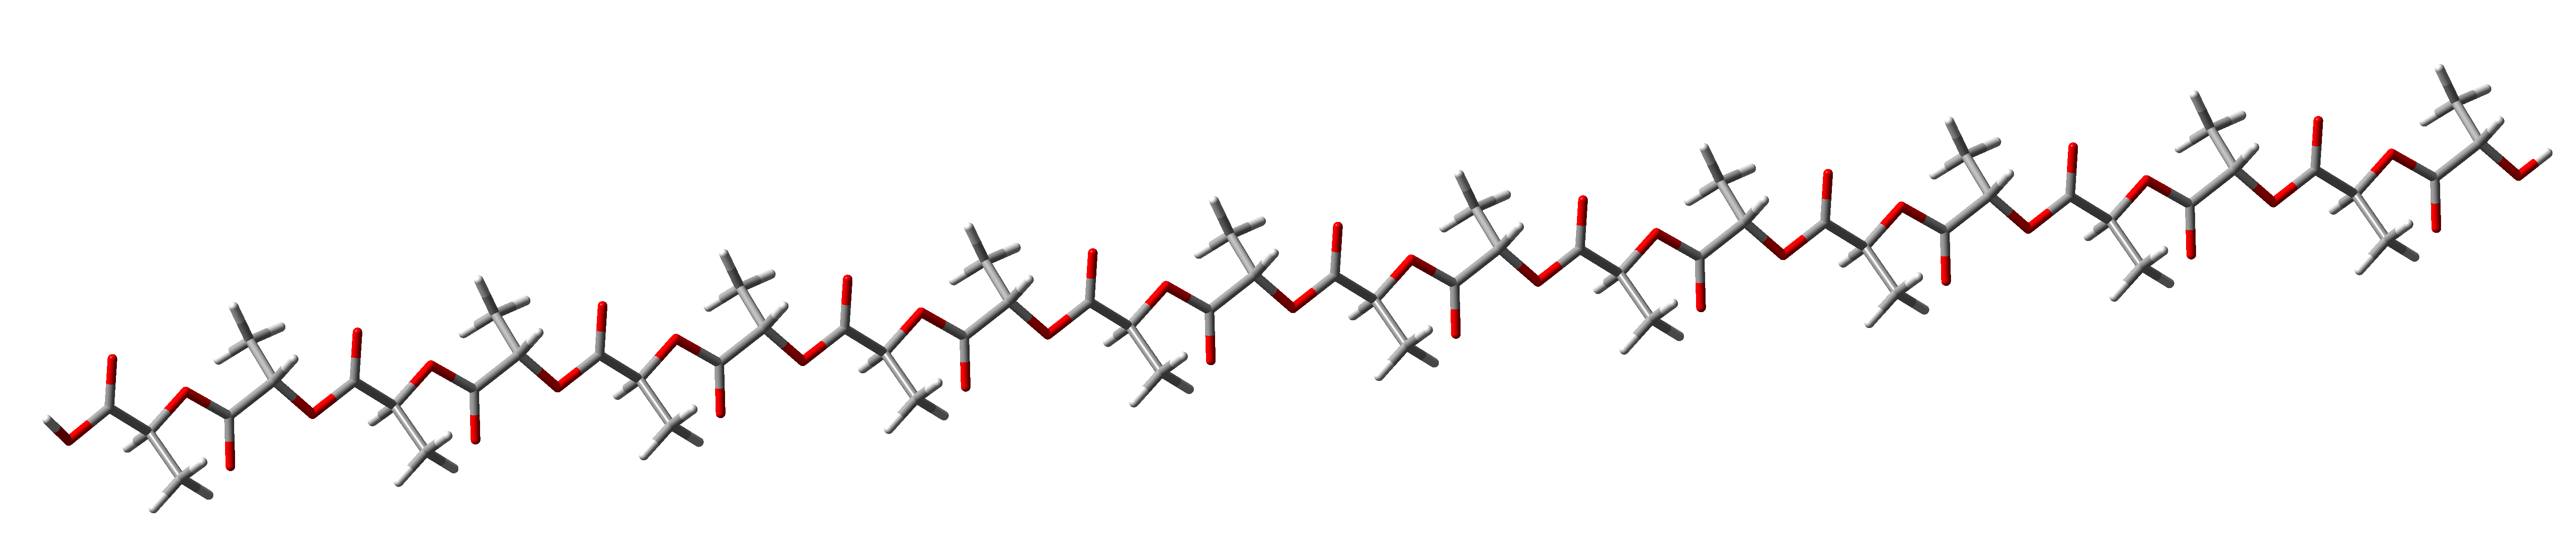
\includegraphics[width=0.9\linewidth]{img/pla_10d_tube.png}
	\caption{Fibrilar PLA polymer chain, 20 units}
	\label{fig:linearni}
\end{figure}

\begin{figure}[htb]
	\begin{subfigure}{0.5\textwidth}
		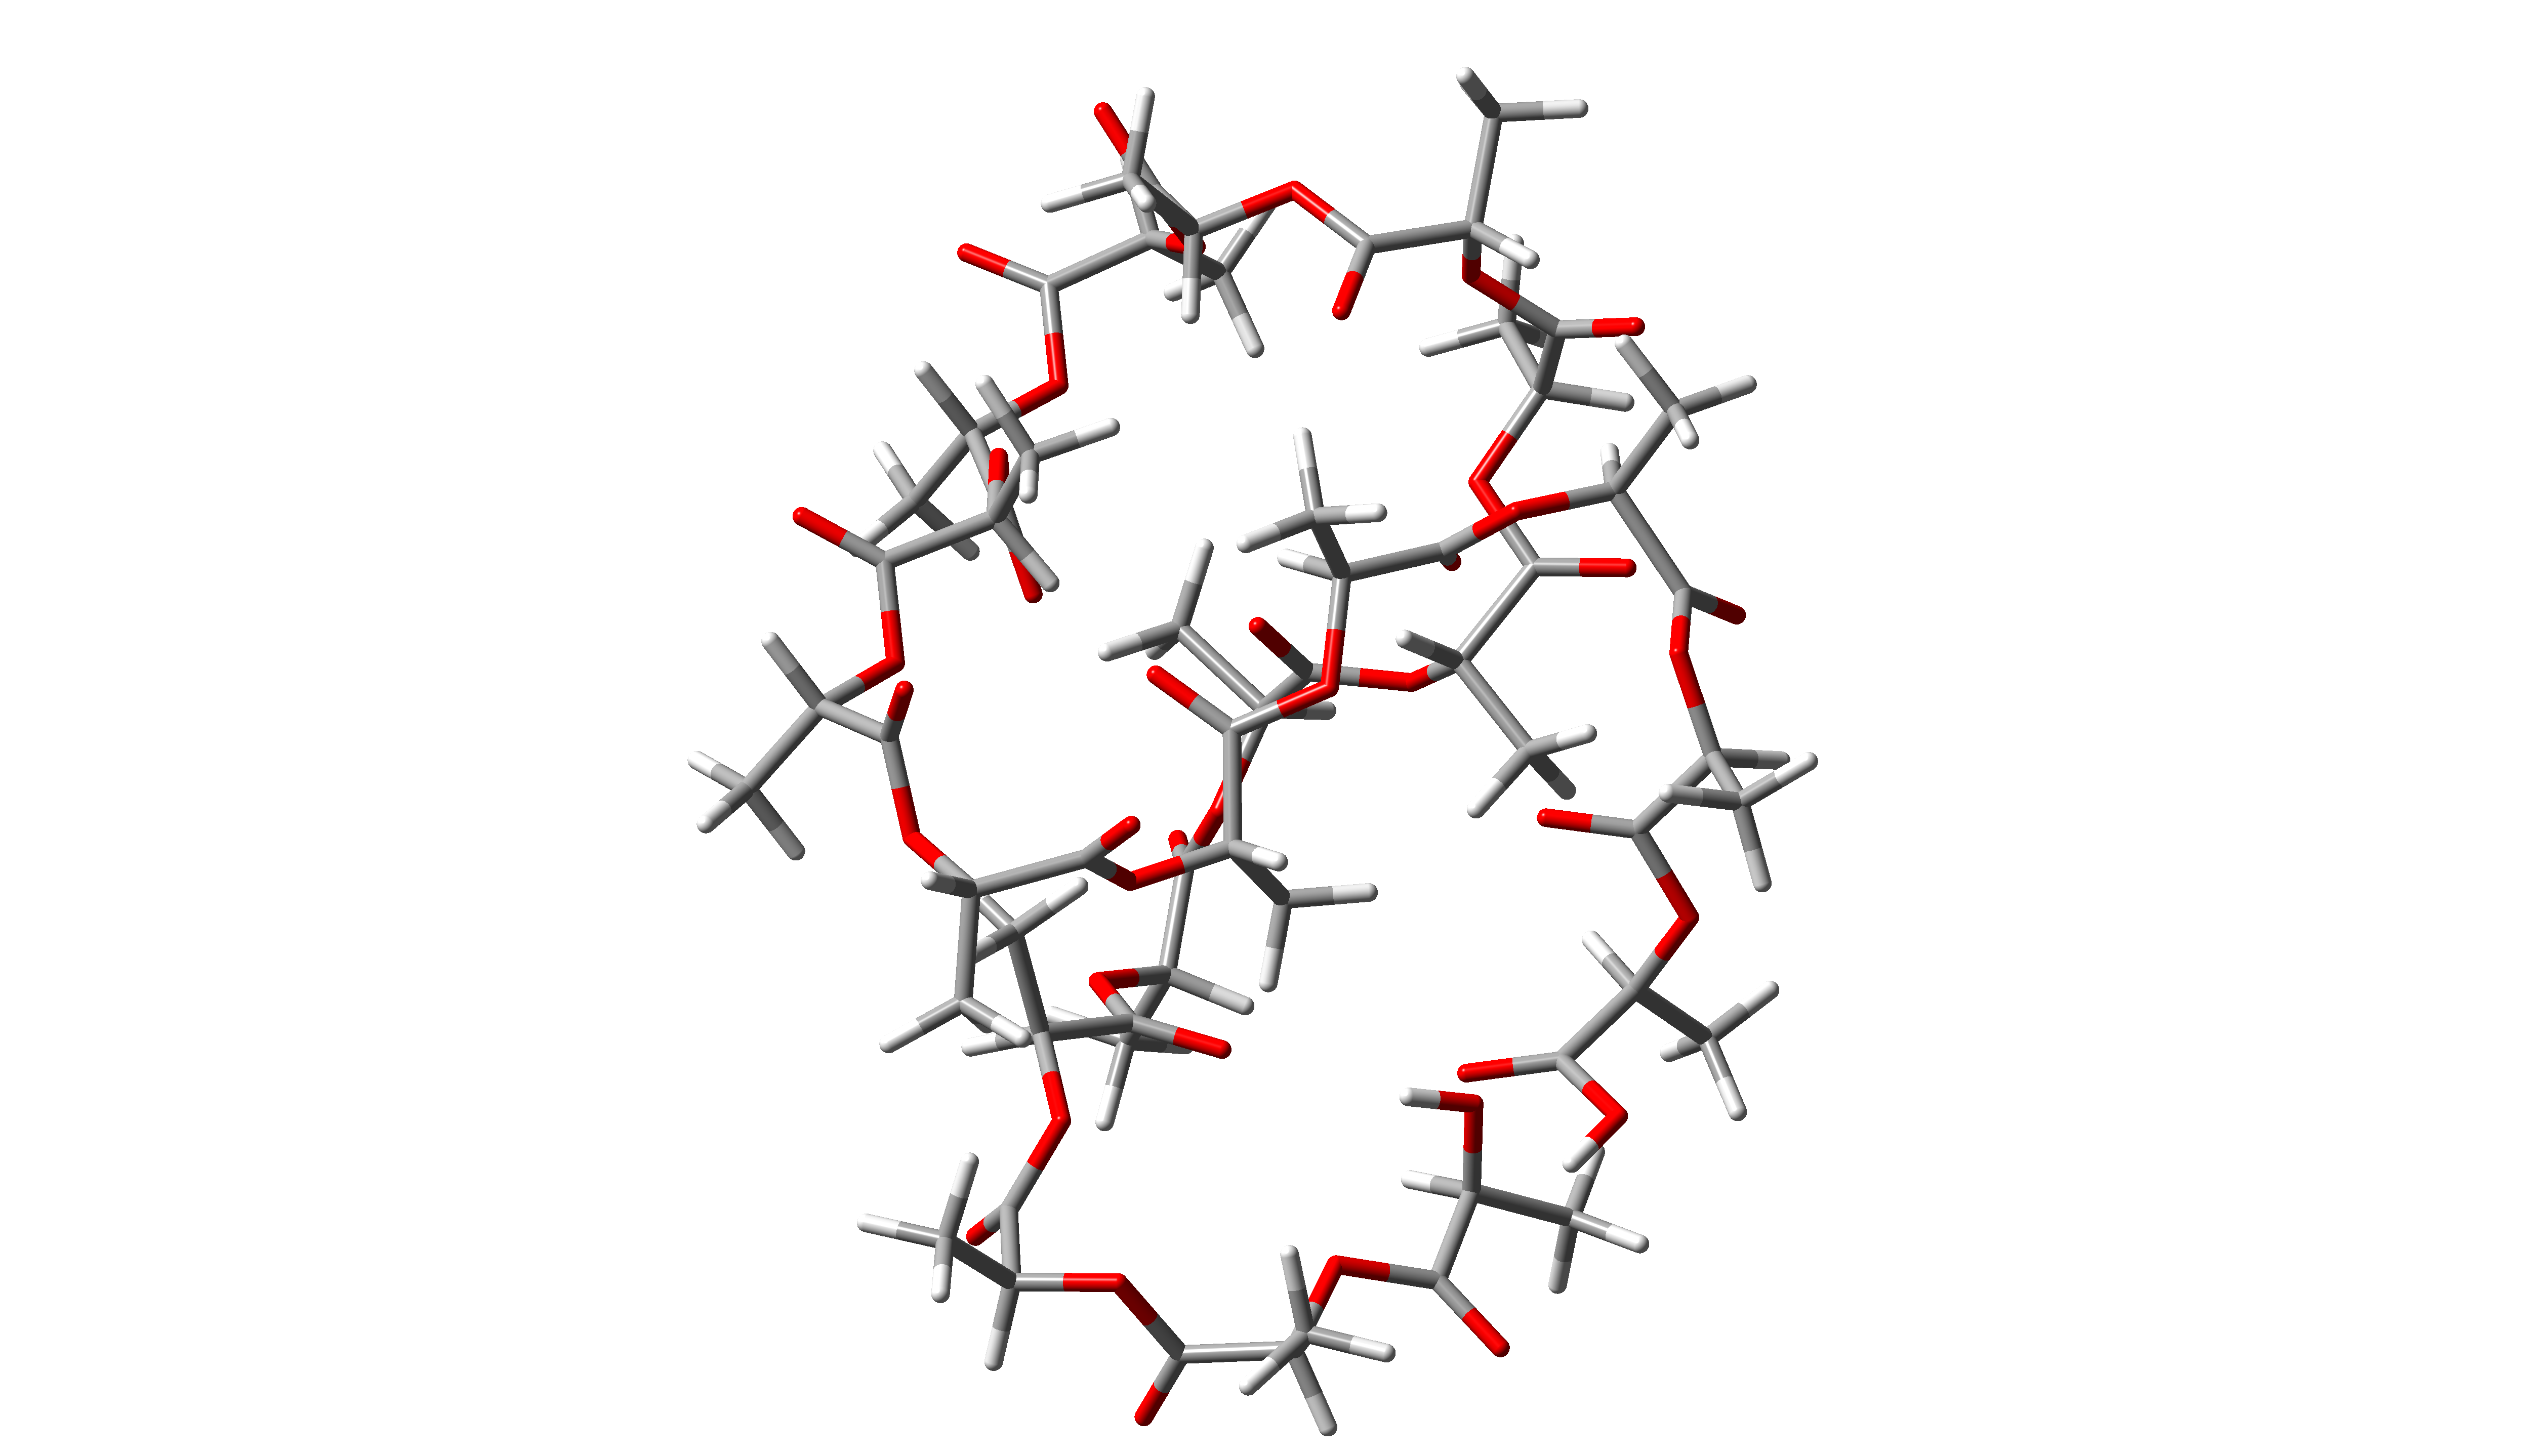
\includegraphics[width=0.9\linewidth]{img/pla_10g_tube.png} 
	\end{subfigure}
	\begin{subfigure}{0.5\textwidth}
		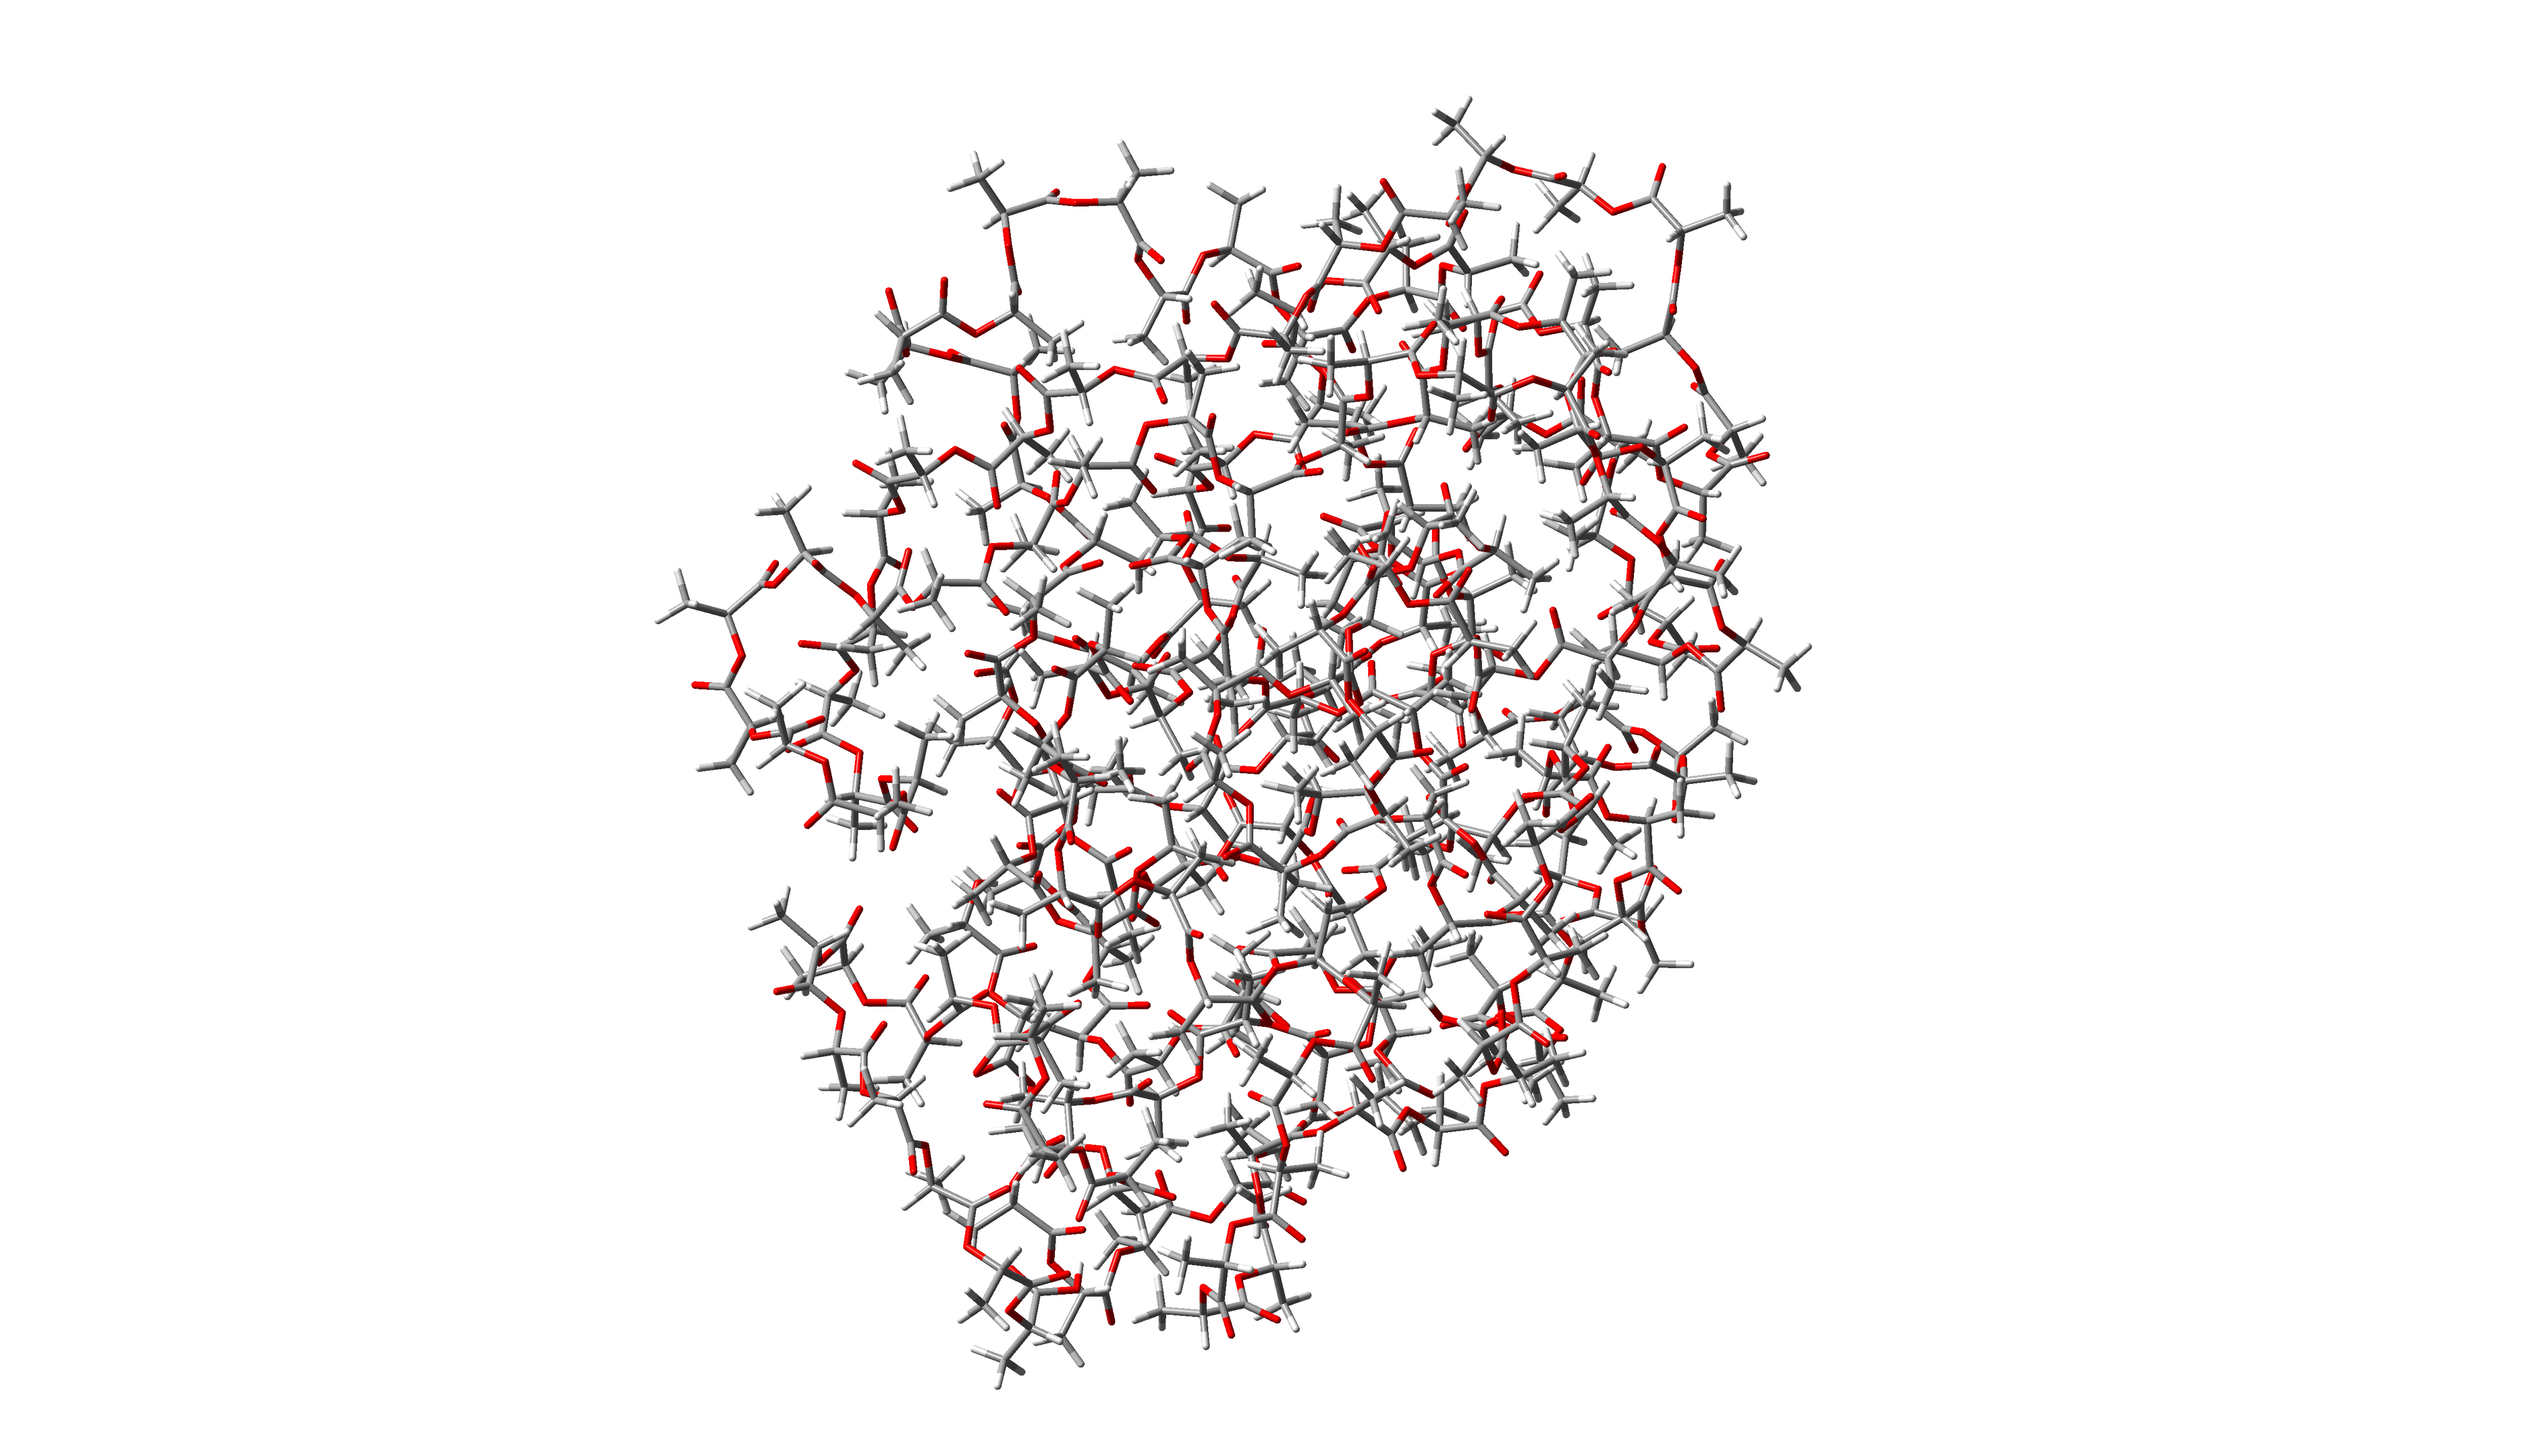
\includegraphics[width=0.9\linewidth]{img/pla_100g_tube.png} 
	\end{subfigure}   	
	\caption{Globular PLA polymer chain, 20 and 200 units}
	\label{fig:sbalene}
\end{figure}

To see the effects of initial conformations, molecular weight and thermal history of the polymer on bulk densities following simulations were performed. The design of the simulation boxes is in Table \ref{tab:pla_chains}. The simulations were first performed at the temperature of 500 K (run 1), then the box was heated up to 1000 K followed by re-cooling and simulating at a temperature of 500 K (run 2). All subsequent simulations were observing the system for 10~ns with a step 1 fs at 1 bar. From these simulations, the densities and the root mean square distance of the polymer chain termini with their standard deviations were evaluated.

\begin{table}[h]
	\centering
	\caption{Design of the neat PLA simulation boxes}
	\label{tab:pla_chains}
	\begin{tabular}{ccccc}
		\toprule
		\textbf{\boldmath$N_{\text{units}}$} & \textbf{\boldmath$n_{\text{chains}}$} & \textbf{\boldmath$N_{\text{atoms}}$} & \textbf{\boldmath$M$, g mol$^{-1}$} & \textbf{\boldmath$d$, \AA} \\
		\midrule
		20 & 140 & 25620 & 1459.3 & 67.9 \\
		40 & 70 & 25410 & 2900.5 & 67.7 \\
		60 & 40 & 24978 & 4341.8 & 64.3 \\
		80 & 35 & 25305 & 5783.1 & 67.7 \\
		100 & 28 & 25284 & 7224.3 & 67.7 \\
		120 & 23 & 24909 & 8665.6 & 67.3 \\
		140 & 20 & 25260 & 10106.8 & 67.6 \\
		160 & 17 & 24531 & 11548.1 & 67.0 \\
		180 & 15 & 24345 & 12989.4 & 66.8 \\
		200 & 14 & 25242 & 14430.6 & 67.6 \\
		\bottomrule
	\end{tabular}
\end{table}

The following graphical representation of the results (Figure \ref{fig:pla_hustoty}) shows a trend of an increasing density depending on the length of the chain (molecular weight), which is independent of the initial conformation of the molecule, the values differs only in . It is also visible that densities for longer chains converge to a constant value. From this finding, we can consider that a system above $M_\mathrm{w}$~=~9~000~$\mathrm{g \ mol^{-1}}$ has reached the polymer limit within the simulation.

\begin{figure}[htb!]
	\begin{subfigure}{0.5\textwidth}
		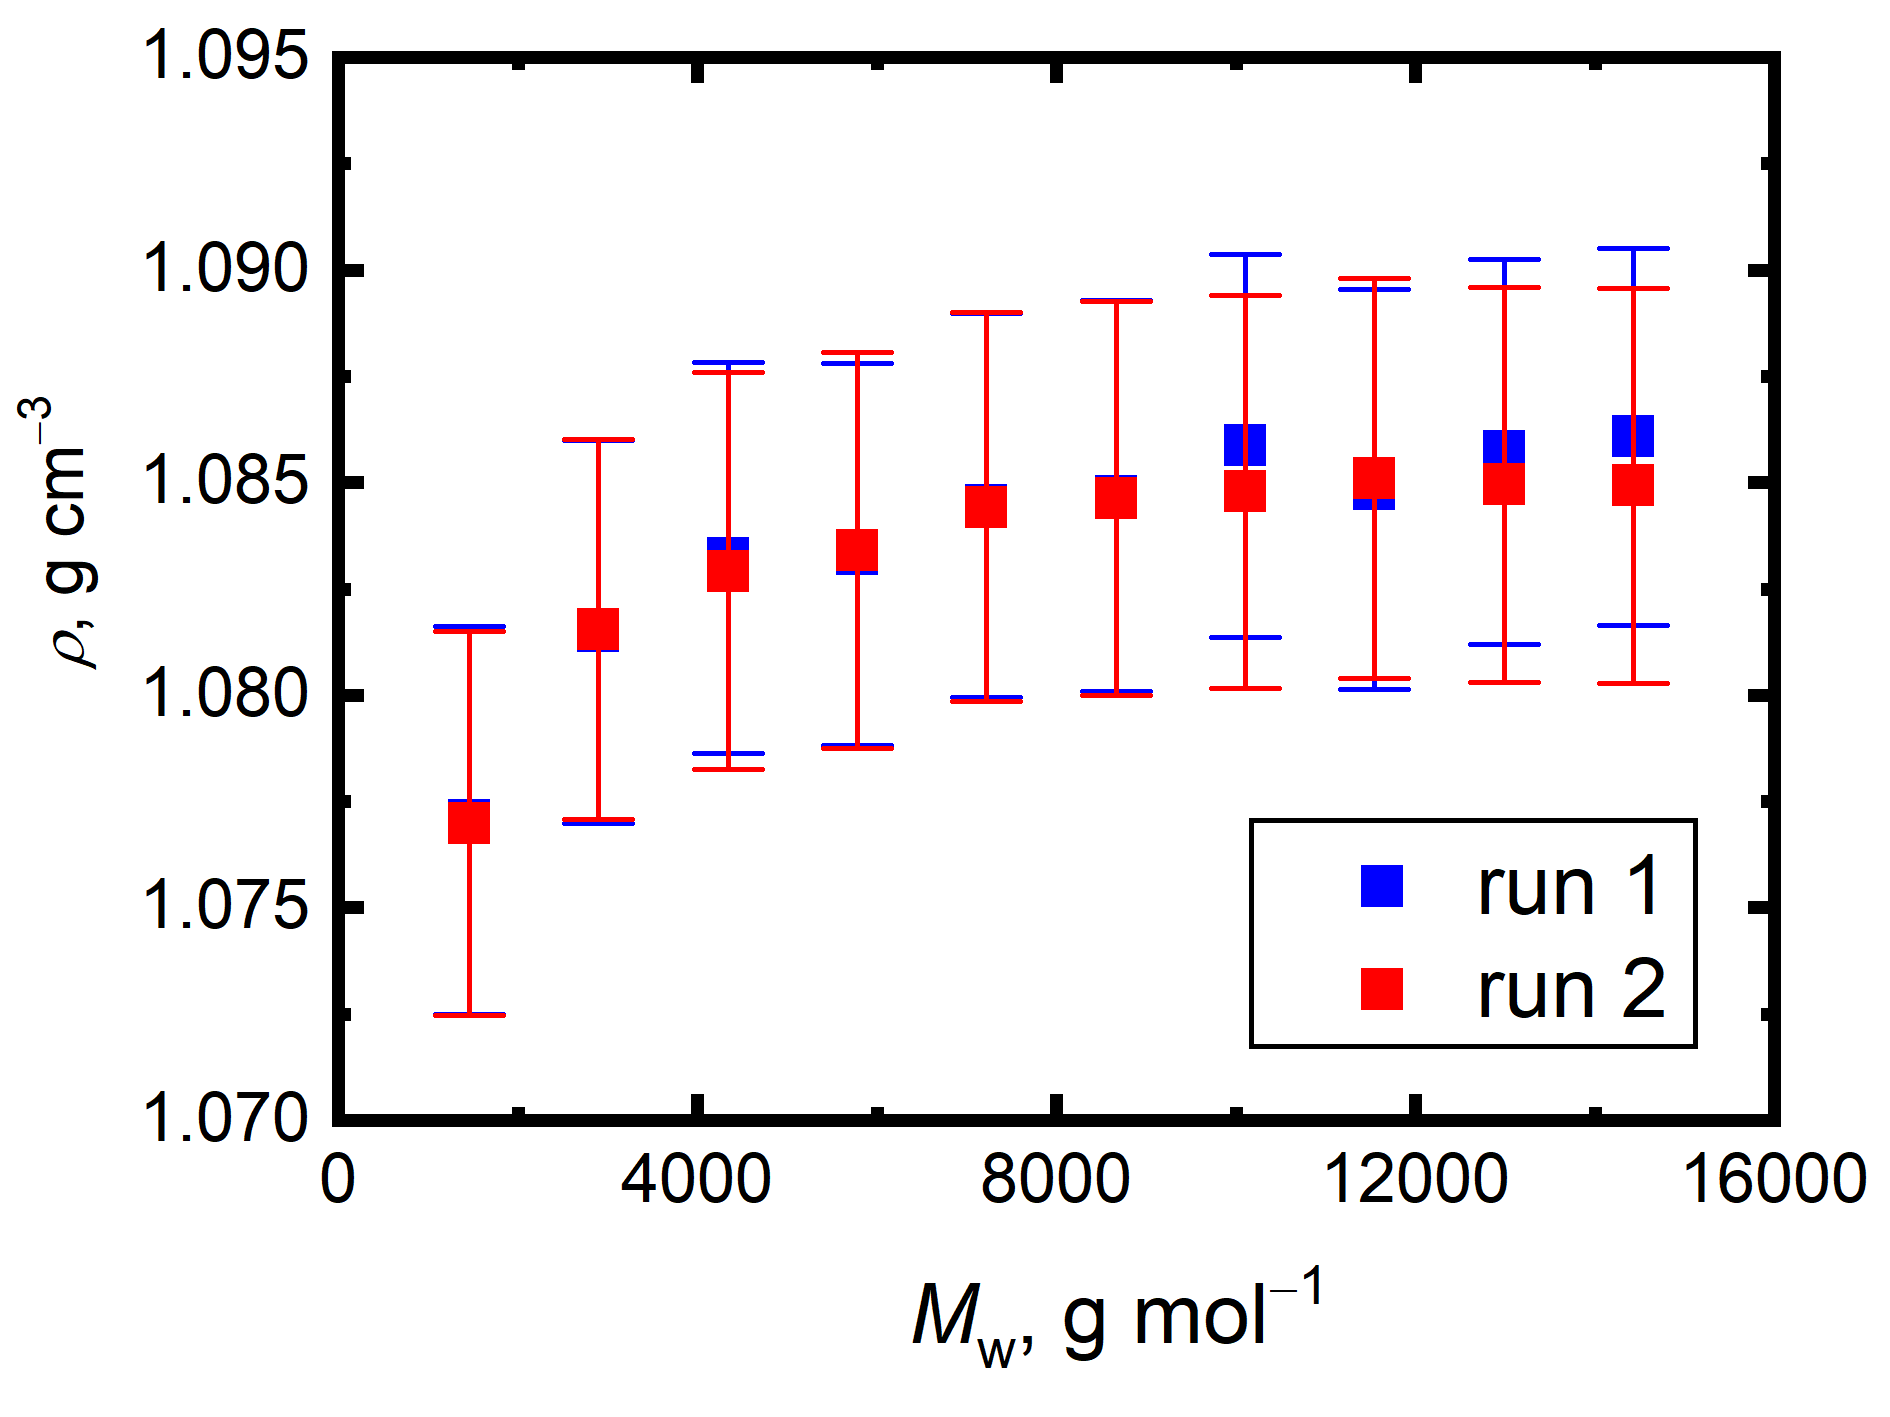
\includegraphics[width=1.0\linewidth]{img/pla_linear_density.png} 
		\caption{from initial fibrilar conformation}
		\vspace{-0.2cm}
	\end{subfigure}
	\begin{subfigure}{0.5\textwidth}
		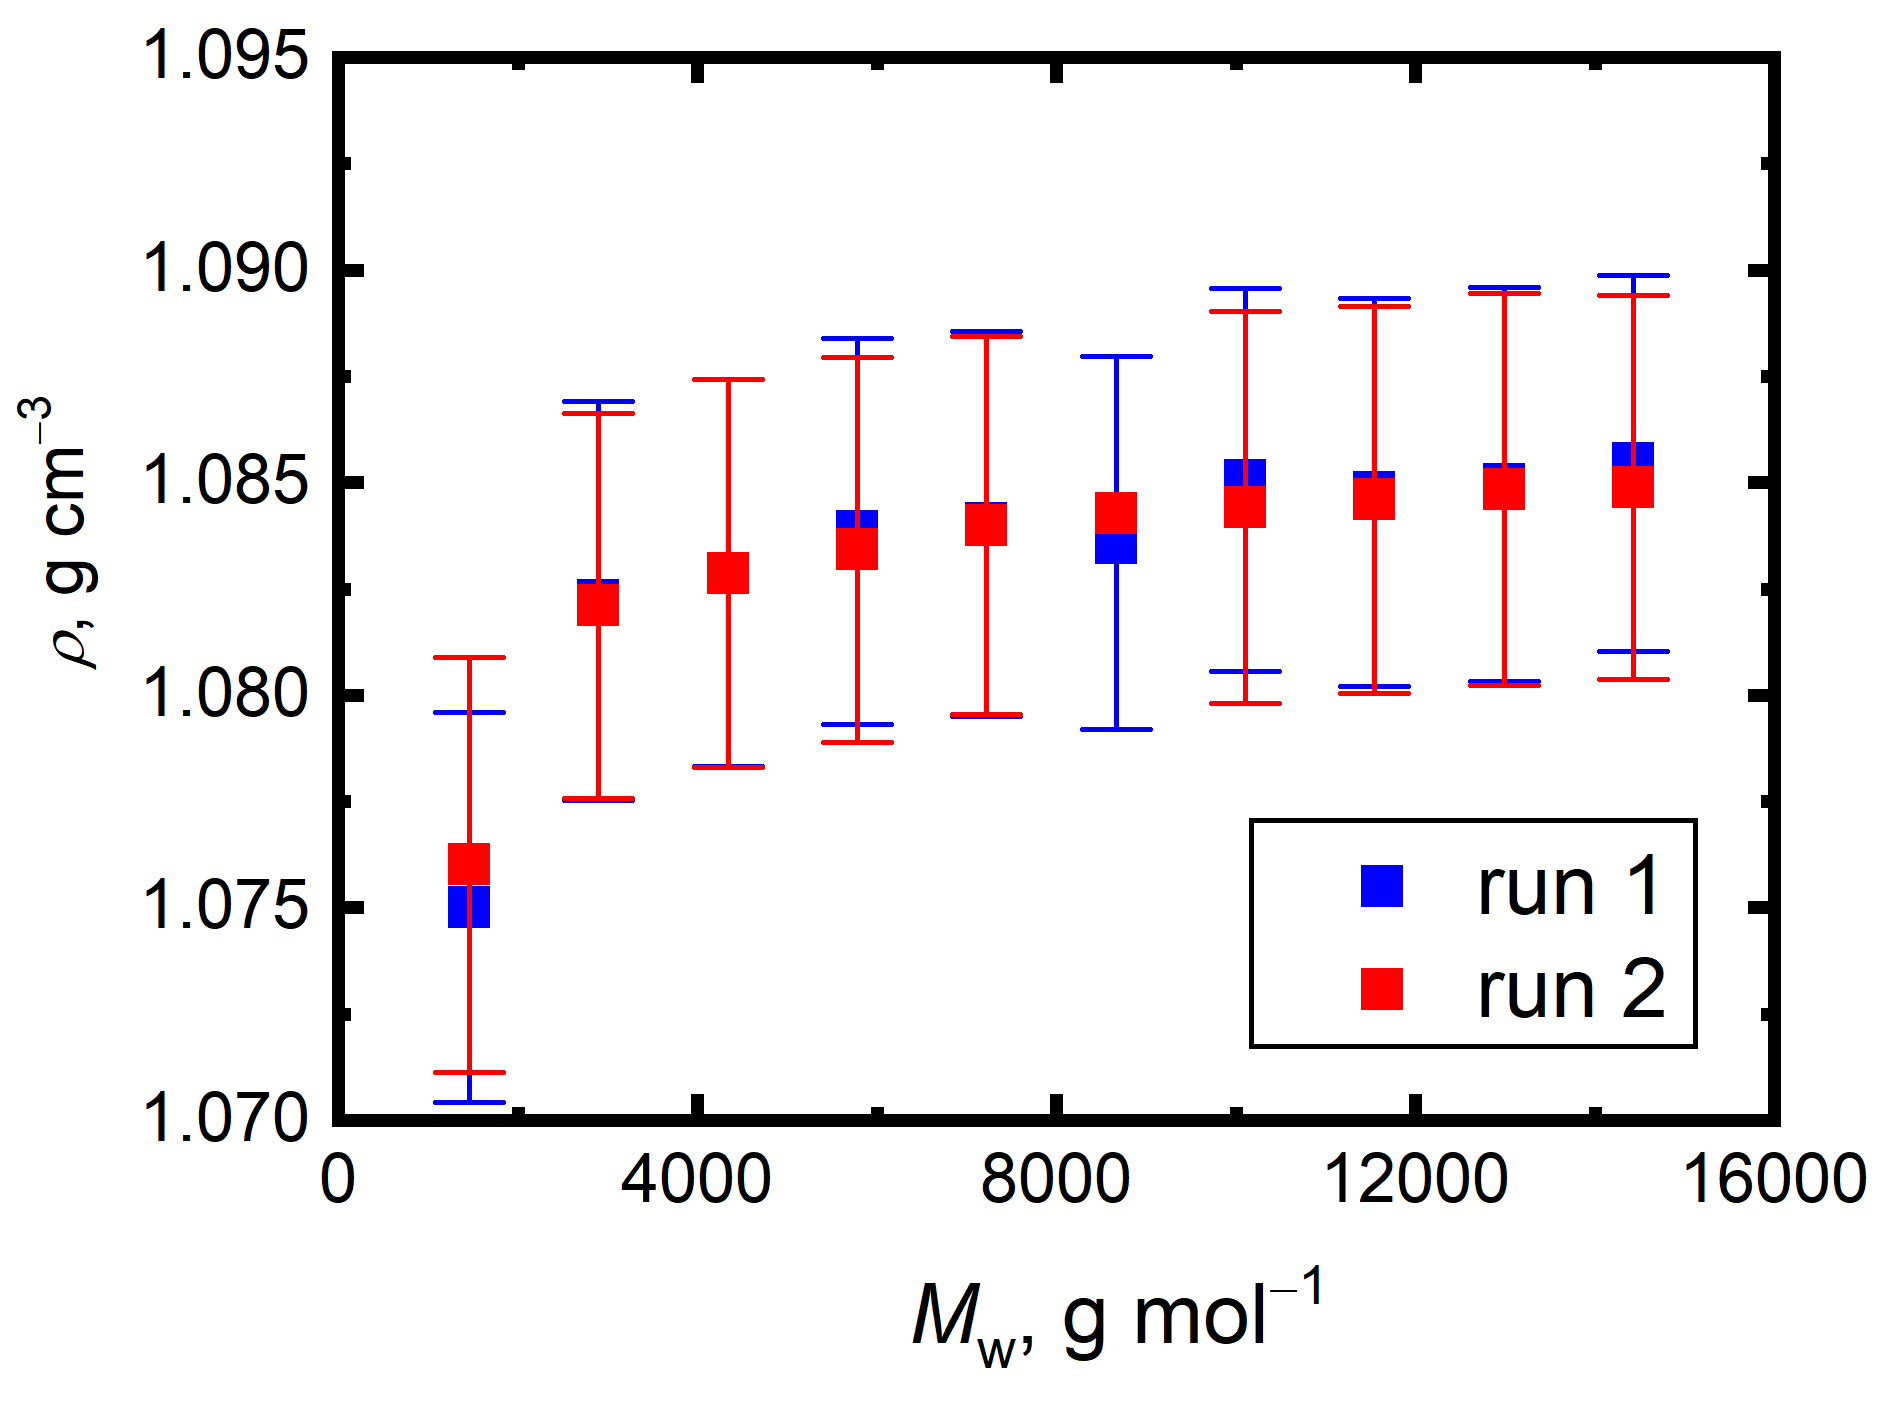
\includegraphics[width=1.0\linewidth]{img/pla_glob_density.png}
		\caption{from initial globular conformation}
		\vspace{-0.2cm}
	\end{subfigure} 
	\caption{Average densities with their standard deviations for PLA polymer chains at 500 K and 1 bar as a function of the chain length before (run 1) heating and (run 2) after cooling.}
	\label{fig:pla_hustoty}
	\vspace{-0.2cm}
\end{figure}

From the density data, any impact of the conformation memory cannot be assessed, since the bulk density is too a crude point of view on the polymer structure. That is the reason why the distances of the polymer chain termini that are displayed in the Figure \ref{fig:pla_konce} were calculated. The simulated time of 10 ns at the elevated temperature 1000 K was not enough to completely erase the polymer conformational memory, there is a noticeable deviation of the data sets obtained from the simulation initiated from the fibrilar and globular conformations.

\begin{figure}[htb!]
	\begin{subfigure}{0.5\textwidth}
		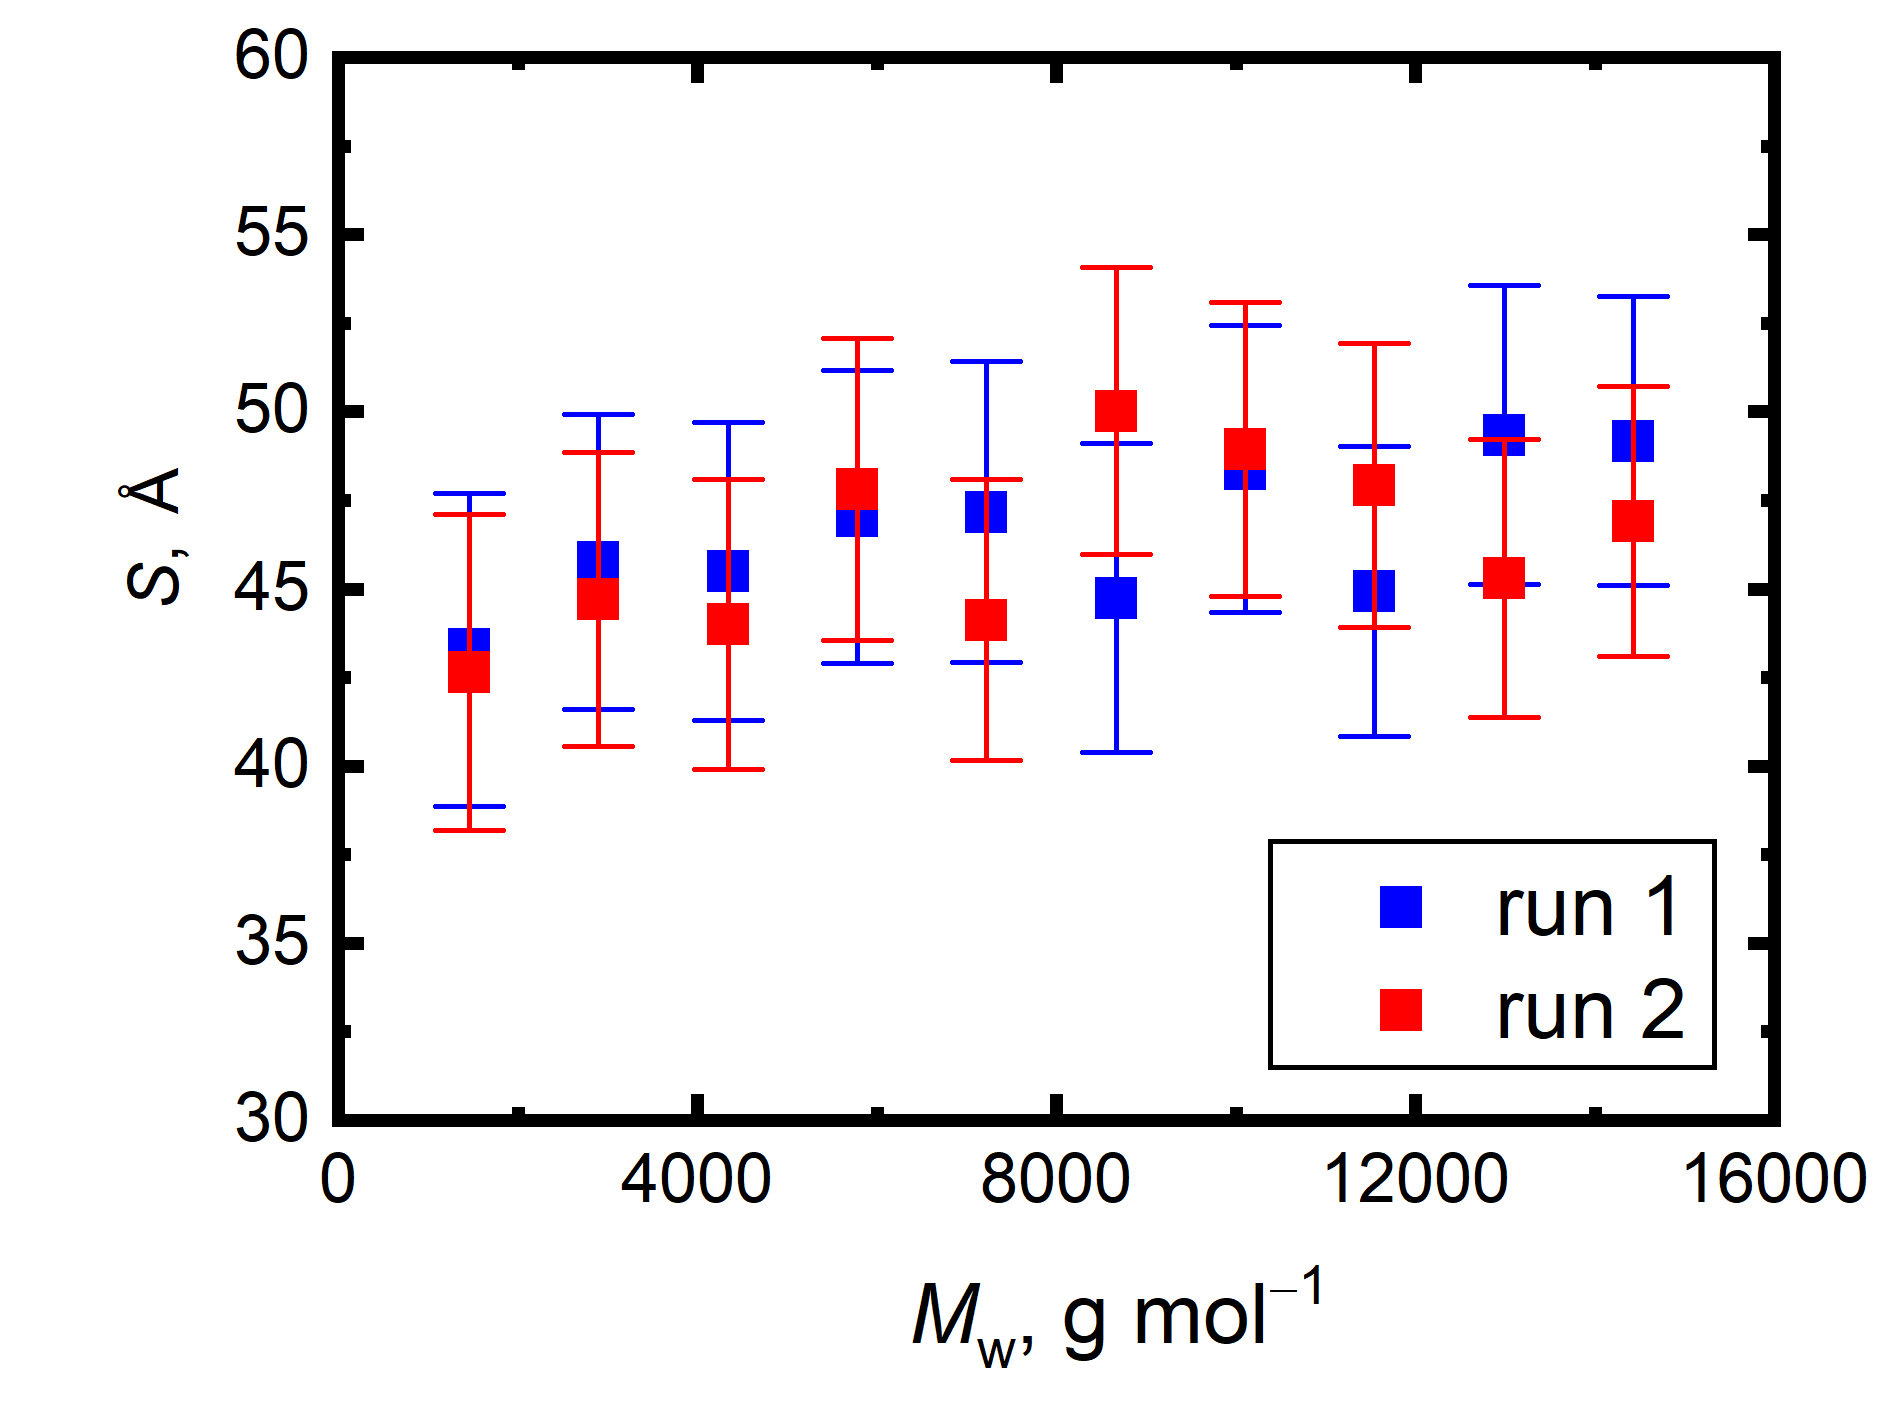
\includegraphics[width=1.0\linewidth]{img/pla_linear_konce.png} 
		\caption{from initial fibrilar conformation}
		\vspace{-0.2cm}
		\label{fig:subim1}
	\end{subfigure}
	\begin{subfigure}{0.5\textwidth}
		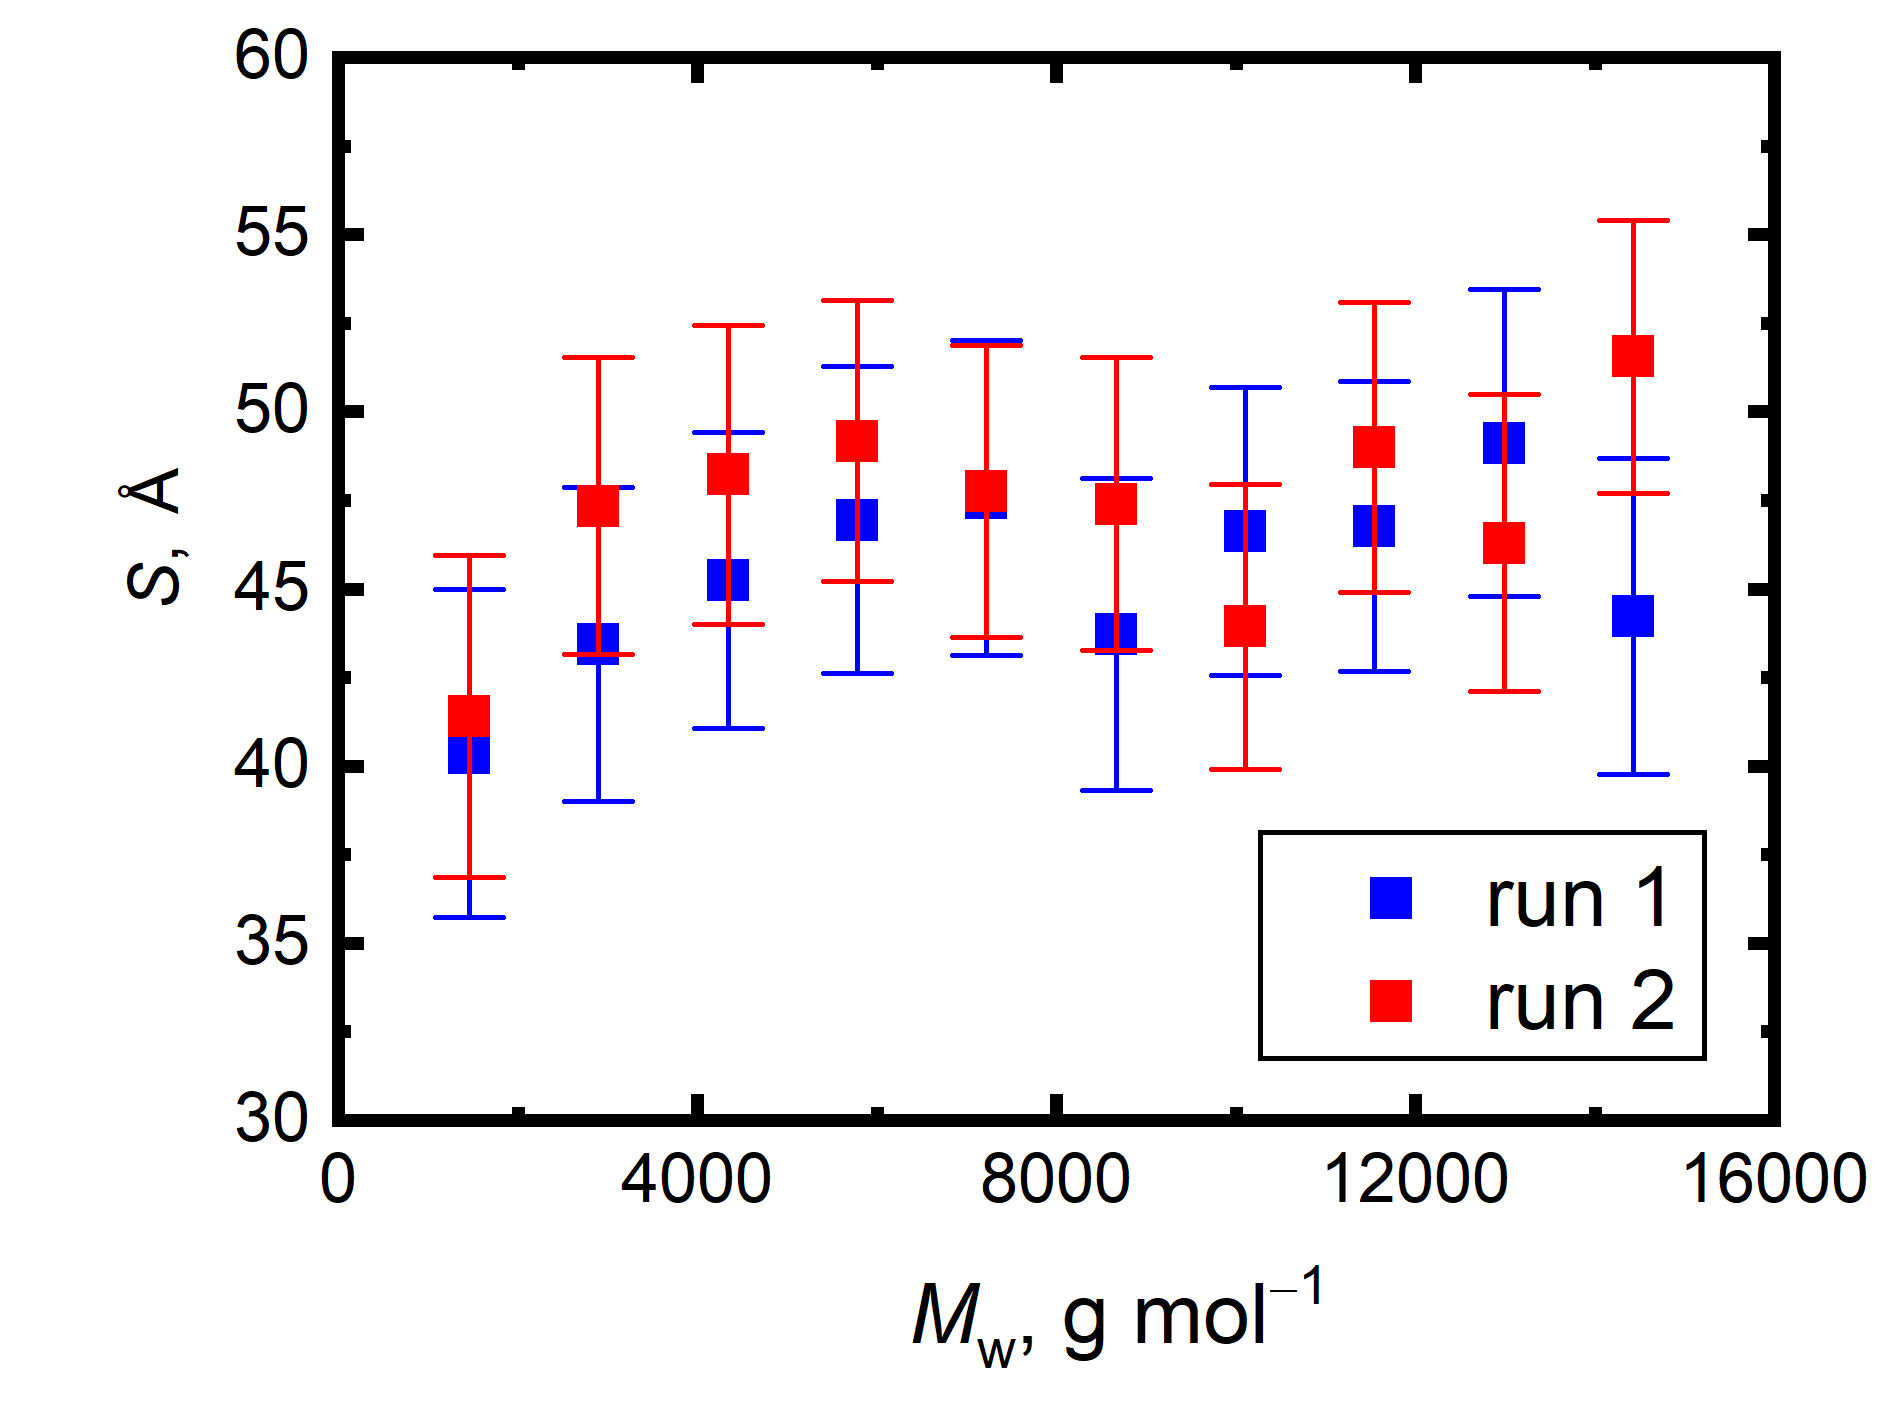
\includegraphics[width=1.0\linewidth]{img/pla_glob_konce.png}
		\caption{from initial globular conformation}
		\vspace{-0.2cm}
		\label{fig:subim2}
	\end{subfigure}
	\caption{Root mean square distances of the polymer chain termini with their standard deviations  for PLA polymer chains as a function of chain length before (run 1) heating and (run 2) after recooling.}
	\label{fig:pla_konce}
\end{figure}      

The dynamics of the polymer is slow due to complex entanglement of individual chains even at elevated temperatures, for a complete loss of the conformational memory it would be necessary to simulate the system for a longer period of time, especially for longer chains.

To investigate the effect of the box size on the molecular simulations, the simulations with boxes containing 5-50 polymer chains inside, each having a molar mass 12 989 $\mathrm{g \ mol^{-1}}$ were performed. The simulations were performed with a 3-block initial equilibration at 1000 K and 1 bar and subsequently cooled to 500 K and simulated for 10 ns. Mean densities obtained from these simulations are shown in the Figure \ref{fig:box} on the left. The simulation results prove that the size of the box has no significant effect on resulting average density. However, there is a visible effect of a lower uncertainty of standard deviations of densities for larger boxes. To have a better insight what is going on the structural level, we also analyzed the root-mean-squared end-to-end distance of the polymer chain termini shown in Figure \ref{fig:box_konce} on the right. From the obtained data, there is visible growing trend in end-to-end distances. That means that the small boxes are not sufficient to represent correctly the distribution of the end-to-end distances in the polymer. We can say, that its value converges for boxes containing more than 40 polymer chains. As a conclusion, when we are focused only on macroscopic properties such as density, we can use smaller number of chains in the simulation boxes in order to save the computational resources. However, when dealing with structural properties, we should be careful and set the number of chains in a simulation box more carefully.

\begin{figure}[htb!]
	\begin{subfigure}{0.5\textwidth}
		\centering
		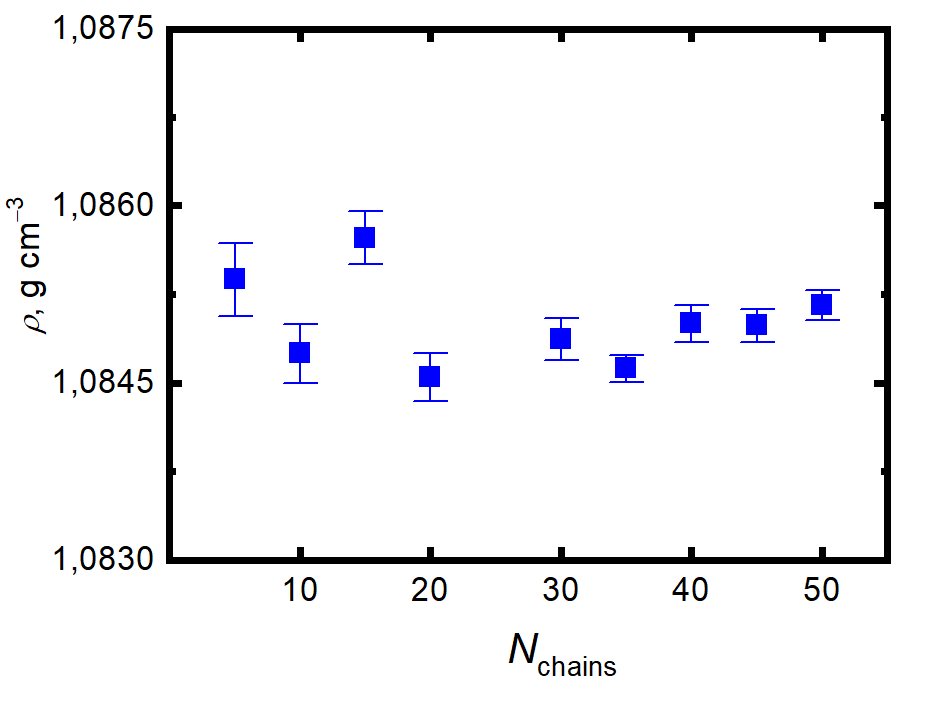
\includegraphics[width=1\linewidth]{img/hustota_5_50_sigma.png}
		\caption{}
		\label{fig:box}
	\end{subfigure}
	\begin{subfigure}{0.5\textwidth}
		\centering
		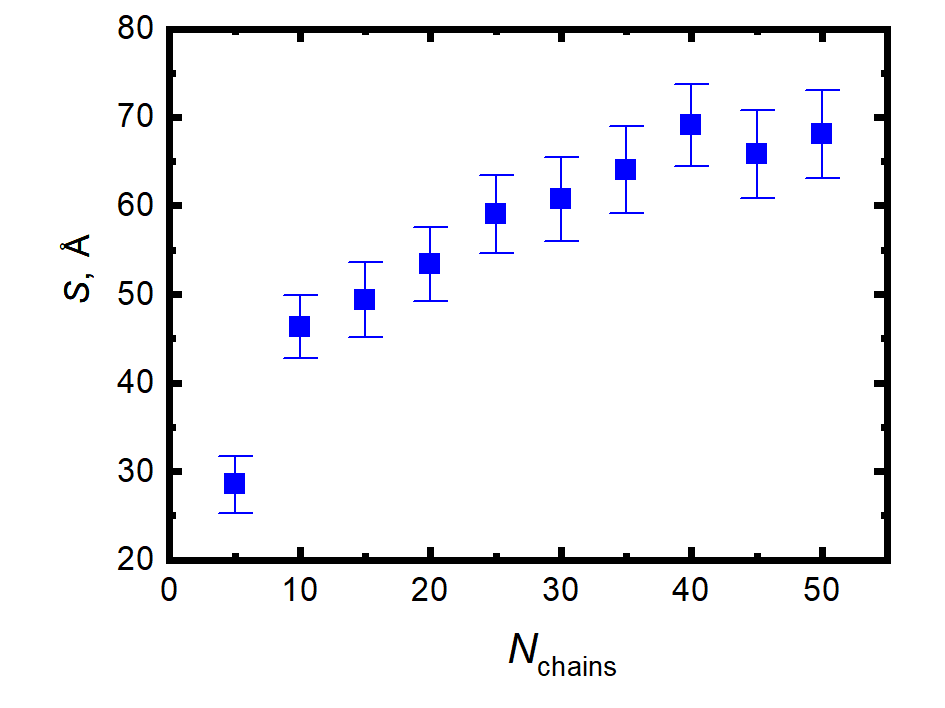
\includegraphics[width=1\linewidth]{img/konce_5_50.png}
		\caption{}
		\label{fig:box_konce}
	\end{subfigure}   	
	\caption{(a) dependence of density on the number of PLA chains containing 90 dimer units in the box on the left and (b) density of PLA at 500 K and 1 bar extracted from MD simulations depending on the polydispersity coefficients on the right.}
	\vspace{-0.2cm}
\end{figure}

To assess the accuracy of the calculated densities, the corresponding experimental data was obtained from literature. The comparison for two temperatures (300 and 500~K) in following Table \ref{tab:PLA_dens} was taken from \cite{klajmon_glass_2023}, where the methodology is also described in more details.

\begin{table}[htbp]
	\centering
	\caption{Comparison of calculated and experimental PLA denstities taken from \cite{klajmon_glass_2023}.}
	\begin{tabular}{ccc}
		\toprule
		$T$, K & $\rho_{\text{exp}},  \text{g cm}^{-3}$ & $\rho_{\text{calc}}, \text{g cm}^{-3}$ \\
		\midrule
		 300   & $1.373 \pm 0.003$ & $1.193 \pm 0.001$ \\
		 500   & $1.181 \pm 0.003$ & $1.086 \pm 0.001$ \\
		\bottomrule
	\end{tabular}%
	\label{tab:PLA_dens}%
\end{table}%

\subsubsection{Polydispersity effect}
Under real conditions, it is hardly possible to experimentally prepare a monodisperse polymer containing only one selected chain length. For this reason, we simulated several polydisperse systems, each exhibiting a different distribution of molar masses of individual molecular chains, containing a total number of 50 chains. Their lengths come from an interval 8-244 units. Polydispersity index PDI~=~1 corresponds to 50 chains of length 124 units, the other values were calculated using the equation \ref{eq:PDI}. We than build composition of the other systems using the Gaussian distribution with the mean value of 124 units. By this procedure, we were able to obtain the PDI up to 1.3. To reach PDI 1.4 and 1.5, we had to increase the numbers of very short and long polymer chains present in the box to get the desired PDI. Designed compositions of systems based on PDI values are displayed in the Figure \ref{fig:polydisperzita_vyskyt}. The density was again evaluated from the simulations, in this case as a function of the PDI.

\begin{equation}
	\text{PDI} = \frac{\sum_{i} N_{i} \cdot \sum_{i} N_{i} M_{i}^2}{\left(\sum_{i} N_{i} M_{i}\right)^2}
	\label{eq:PDI}
\end{equation}


\begin{figure}[htb]
	\centering
	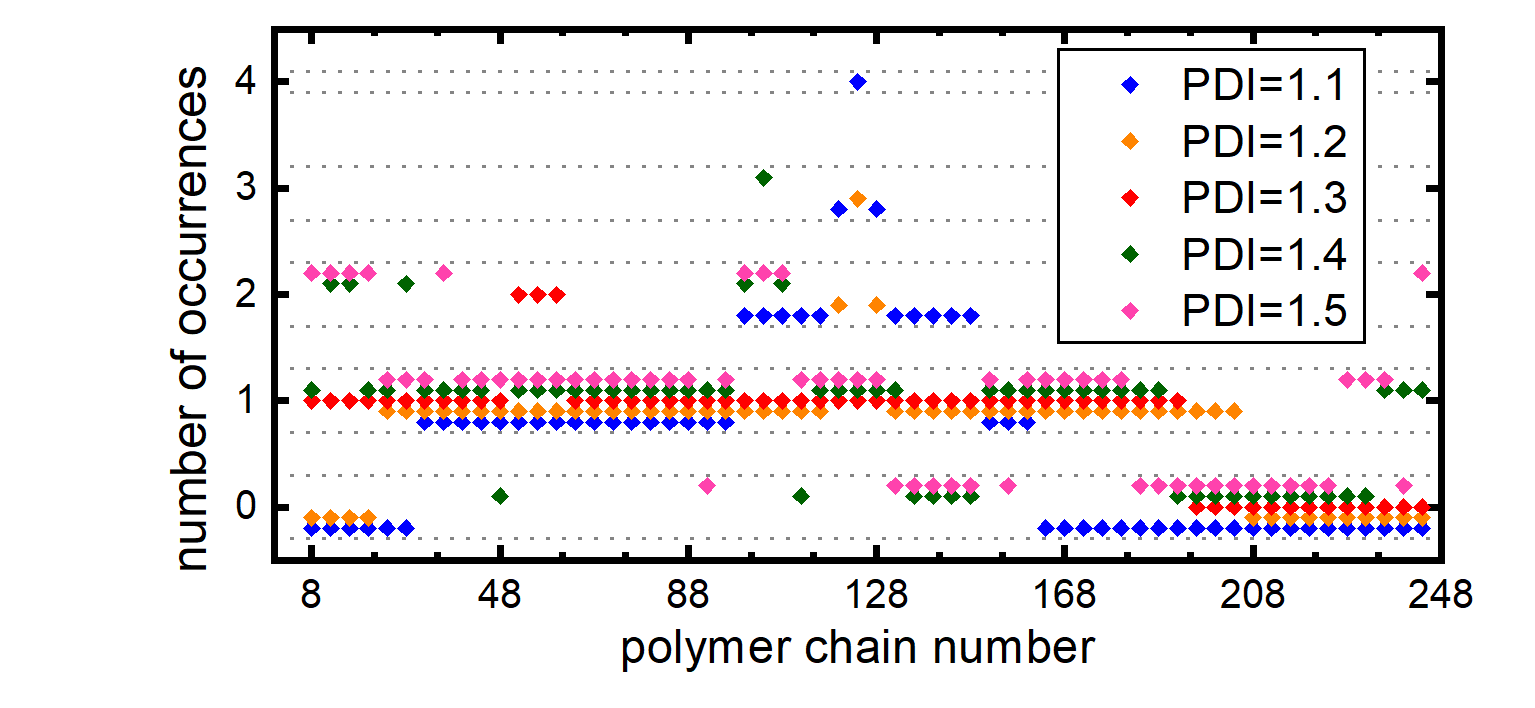
\includegraphics[width=1\hsize]{img/polydispersity_occurences_new.png}
	\caption{Number of occurrences of chains of a given length in the polydisperse systems with corresponding PDI.}
	\label{fig:polydisperzita_vyskyt}
\end{figure}       

Calculated densities depending on the PDIs are in the Figure \ref{fig:polydisperzita}. There is no significant difference among the densities obtained for different values of the polydispersity index. For the subsequent simulations we will use monodisperse systems as it will not introduce deviations from macroscopic behavior. 

\begin{figure}[htb]
	\centering
	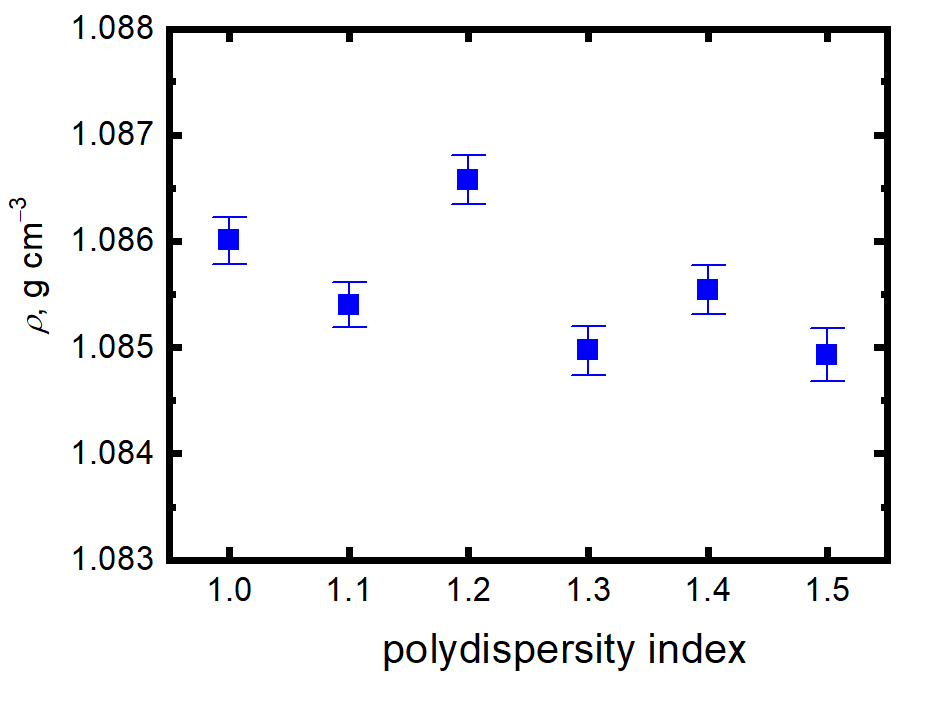
\includegraphics[width=0.5\hsize]{img/polydisperzita_new.png}
	\caption{Density of PLA at 500 K and 1 bar extracted from MD simulations depending on the polydispersity coefficients.}
	\label{fig:polydisperzita}
\end{figure}       

\subsubsection{Glass transition modeling}
Understanding the glass transition temperature of pharmaceutical materials is crucial for drug formulation, storage, and delivery. The $T_\text{g}$ refers to the temperature at which an amorphous material transitions from a rigid, glassy state to a more flexible, rubbery state without melting. The knowledge of $T_\text{g}$ helps us predict and control the stability of drugs during long-term storing.  

To obtain the glass transition temperature of PLA ($T_\mathrm{g}$), we started by simulating ten different polymer chain lengths for a set of temperatures in a range 140-485 K with a step of 15 K. For the system equilibration, each polymer chain simulation ran for 1 ns with a step of 1 fs. After the equilibration, the temperature interval for the following simulations was limited to the range of 200-485 K with a step of 15 K. Then, we run a $NpT$ production simulation for each temperature with this limited interval for 10 ns with a step of 1 fs from which the equilibrium bulk phase densities were calculated and displayed as a function of temperature. To get the glass transition temperature ($T_\mathrm{g}$) for PLA from volumetric data, the trend shift method was used \cite{klajmon_does_2022}. 

The trend shift method is illustrated for one length of the polymer chain in the Figure \ref{fig:glass}. When we plot the bulk phase densities as a function of temperature, there is a visible trend shift which has the meaning of the transition between the glassy state and the rubbery state of a polymer. The point of the transition divides the density dataset into two intervals. Coordinates of the breakpoint and one surrounding point from each side were excluded from the further processing and the two resulting intervals were interpolated by a linear function. The $x$-coordinate of the intersection of these two lines determines the glass transition temperature. For this purpose a script in Maple software solving the system of linear equations was created to get the $T_\mathrm{g}$.

Available experimental $T_\mathrm{g}$ of L-PLA varies in the literature, the value  of $T_\mathrm{g}$ = 333 $\pm$ 4~K \cite{pyda_reversing_2005} was chosen. Our obtained PLA $T_\mathrm{g}$ = 337 $\pm$ 10~K as an arithmetic mean of the values for all polymer chain lengths. The calculated $T_\mathrm{g}$ for each polymer chain are displayed as function of polymer chain weight in the Figure \ref{fig:glass} with their arithmetic mean value drawn as a blue line. The calculated $T_\mathrm{g}$ value is very close to the experimental one. There is no significant trend in $T_\mathrm{g}$ of PLA from the calculated data. 


\begin{figure}[H]
	\begin{subfigure}{0.5\textwidth}
		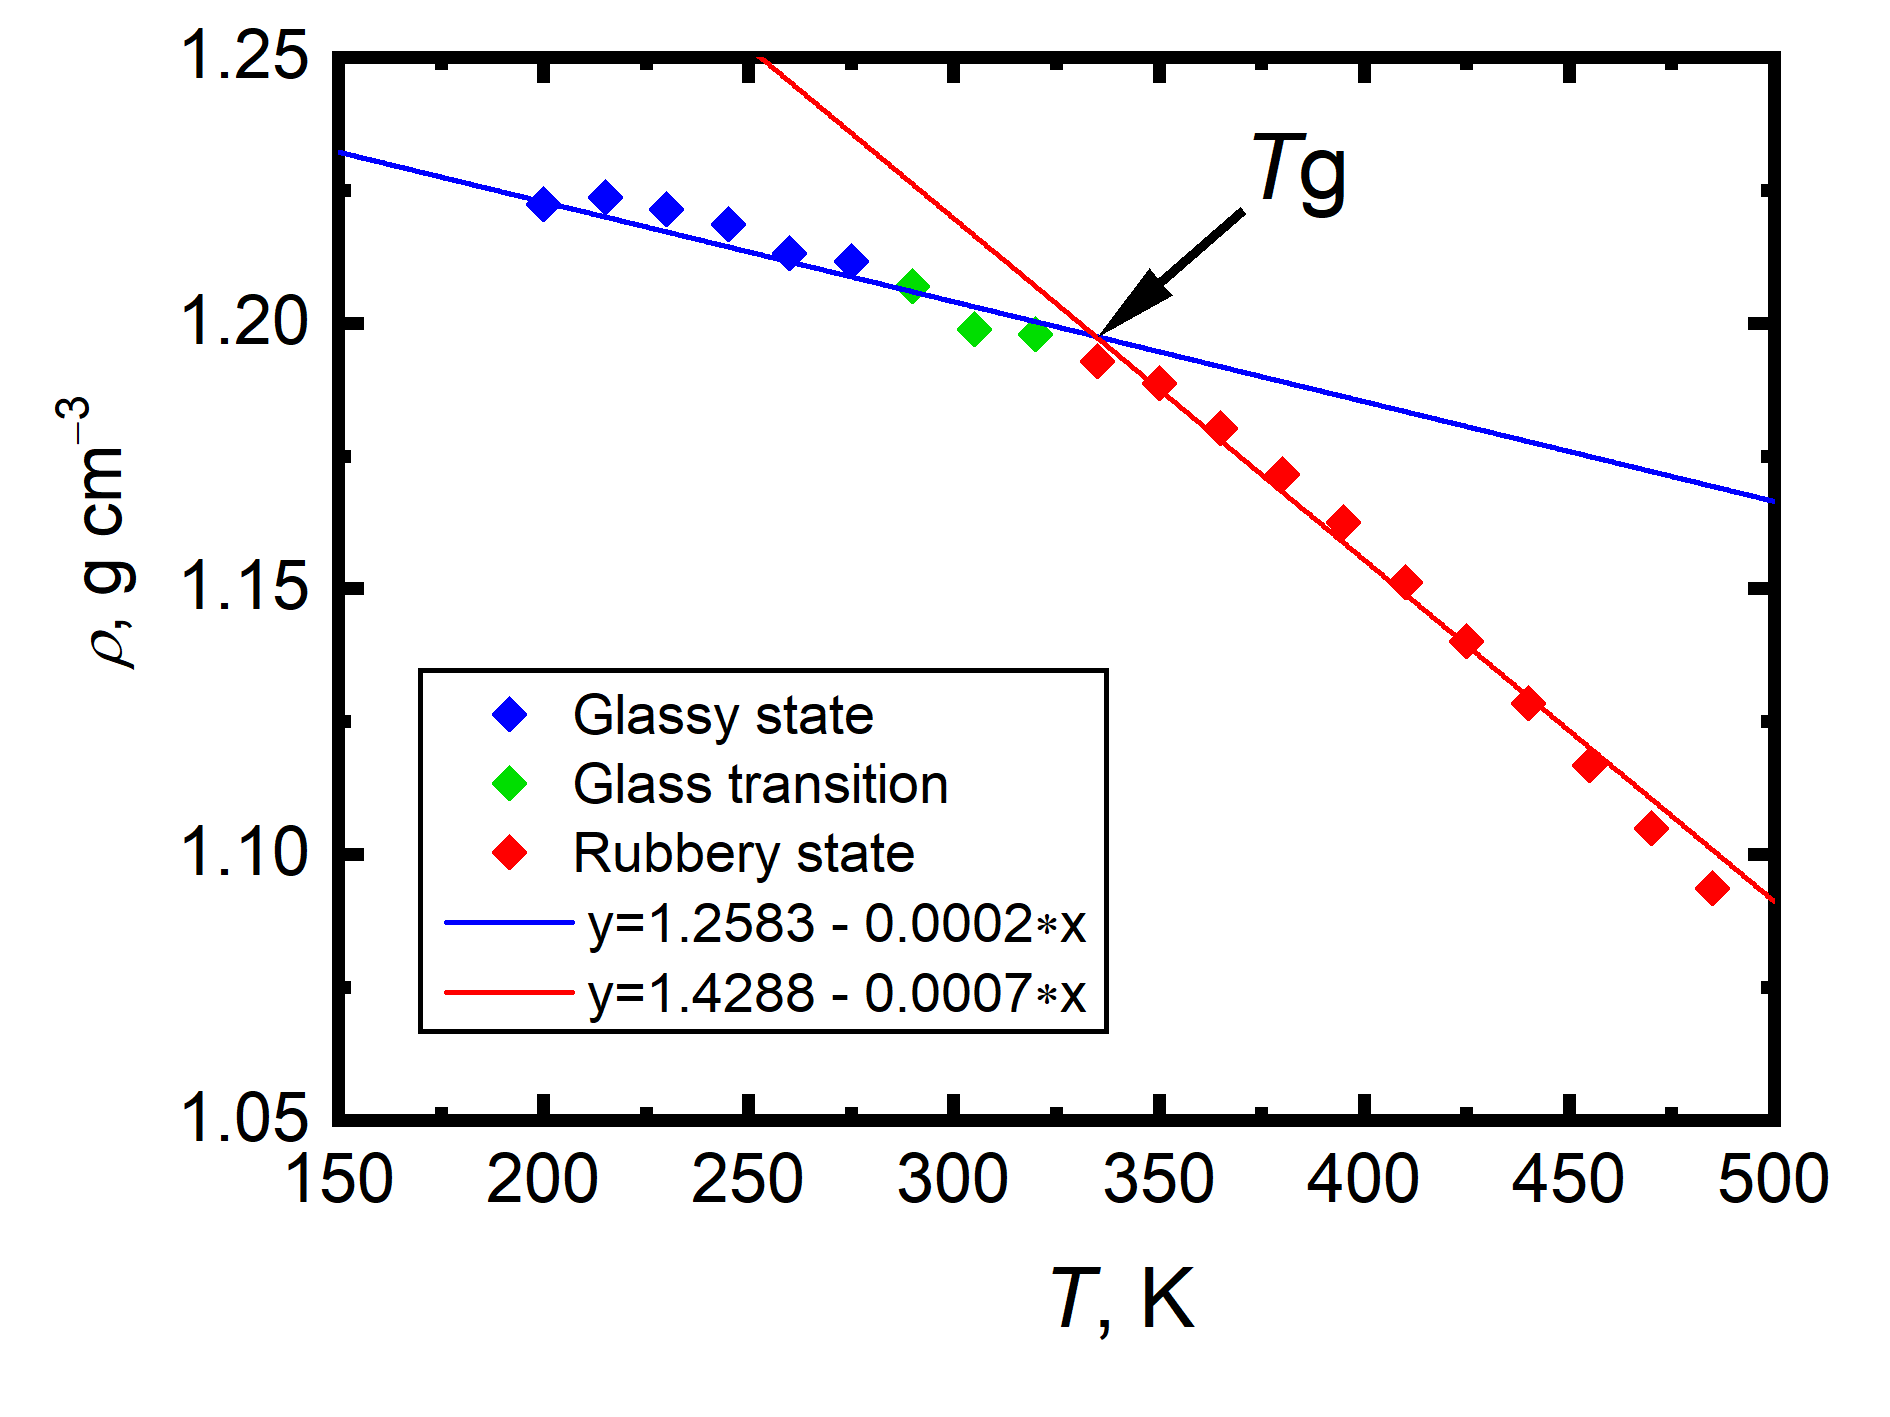
\includegraphics[width=1.0\linewidth]{img/vypocet_tg.png} 
	\end{subfigure}
	\begin{subfigure}{0.5\textwidth}
		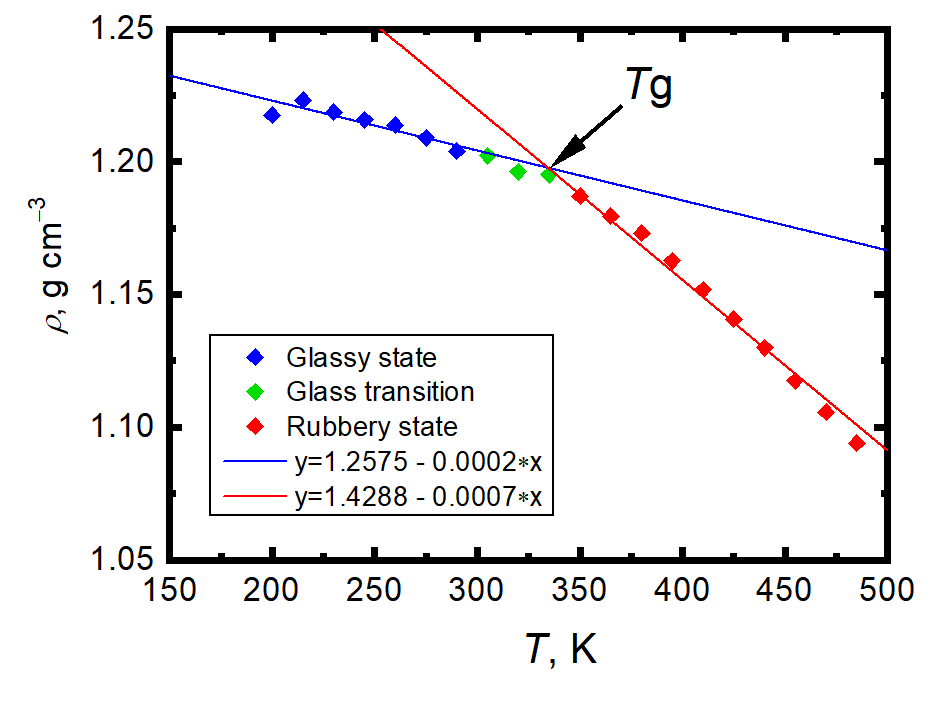
\includegraphics[width=1.0\linewidth]{img/tg_ukazka_30.png} 
	\end{subfigure}   	
	\vspace{-1cm}
	\caption{Illustration of the trend shift method for one polymer chain length on the left, and calculated $T_\mathrm{g}$ for all lengths of polymer chains by this method where blue line represents mean value on the right.}
	\label{fig:glass}
\end{figure}

\newpage
\subsection{Simulations of neat API}
The parameters of API simulation boxes after the equilibration run ($T$=500 K) are presented in Table \ref{tab:API_n}, showing the number of API molecules ($N_{\text{API}}$), the total number of all atoms ($N_{\text{atoms}}$) and size of the cubic box ($l_{\text{box}}$).

\begin{table}[htb!]
	\caption{Properties of equlibrated simulations boxes for bulk API one-component systems, $T$=500 K.}
	\centering
	\begin{tabular}{lcccc} \toprule
		{\textbf{API}} & {\textbf{\boldmath{$N_{\text{API}}$}}} & \textbf{{\boldmath{$N_{\text{atoms}}$}}} & \textbf{{\boldmath{$M$, g mol$^{-1}$}}} & \textbf{{\boldmath{$l_{\text{box}}$, \AA}}} \\
			\midrule
			carbamazepine  & 800 & 24 000 & 236.27 & 66 \\		
			naproxen  & 800 & 24~800 & 230.26 & 66 \\
			ibuprofen  & 800 & 26~400 & 206.28 & 67 \\
			indometacine  & 600 & 24~600 & 357.8 & 66 \\
			\bottomrule
		\end{tabular}
		\label{tab:API_n} 
	\end{table}
	
	To validate the force fields, computed densities were compared with experimental literature values, the comparison is in the Table taken from literature. UPRAVÍM \cite{cervinka_structure_2021}
	
	\begin{figure}[htb!]
		\centering
		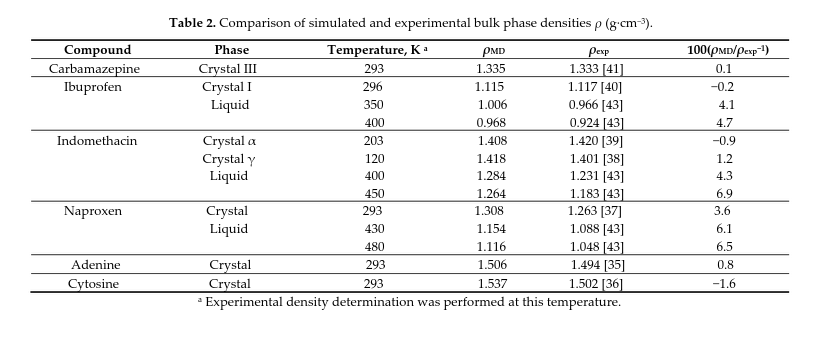
\includegraphics[width=1.0\linewidth]{img/tabulka_validace.png}
	\end{figure}

\subsubsection{Sulfathiazole FF parametrization}
A newly parametrized force field \cite{jorgensen_development_1996} was used for sulfathiazole. The charges on the atoms were calculated by quantum-chemical calculations using the Gaussian code \cite{frisch_gaussian16_2016}. At first, the structure was optimized using the B3LYP functional with the aug-cc-pVTZ basis set with the dispersion correction GD3BJ \cite{smith_revised_2016}. After finding the optimal geometric structure of the molecule, the charges on the atoms were fitted through the CHELPG (Charges from ELectrostatic Potentials using a Grid-based method) method and inserted into force field file.
 
The MD simulations of the sulfathiazole crystal were performed to validate the force field file parameters. The triclinic simulation box and barostat setting was used to account for the anisotropic character of the molecular crystal, other settings are similar to that with the PLA instead of calculating long-range interactions. The sulfathiazole crystal was simulated for three temperatures of 100, 200 and 300 K at 1 bar. The simulation results and experimental data obtained from literature \cite{drebushchak_crystal_2008} are given in the Table \ref{tab:sulfathiazol}.
 
    \begin{table}[htb]       
	\centering
	\begin{tabular}{lccc}
		\toprule
		Temperature, K & 100 & 200 & 300\\
		\midrule
		Experimental density $\rho_\mathrm{exp}$, g cm$^{-3}$  & $1.575 \pm 0.002$ & $1.560 \pm 0.002$ & $1.540 \pm 0.002$\\
		Calculated density $\rho_\mathrm{MD}$, g cm$^{-3}$ & $1.552 \pm 0.001$ & $1.534 \pm 0.002$ & $1.515 \pm 0.002$\\
		100($\rho_\mathrm{MD}/\rho_\mathrm{exp}-1$) & $-1.5$ & $-1.7$ & $-1.6$\\
		\midrule
		Experimental $\beta$ angle, $^{\circ}$ & $94.14$ & $93.905$ & $93.674$\\
		
		Calculated $\beta$ angle, $^{\circ}$ & $91.56$ & $91.64$ & $91.67$\\
		
		Calculated cell a length, \AA & 8.302 & 8.325 & 16.701\\
		
		Calculated cell b length, \AA & 8.236 & 8.275 & 16.625\\
		
		Calculated cell c length, \AA & 7.995 & 8.027 & 16.133\\
		\bottomrule
	\end{tabular}
	\caption{Comparison of simulated and experimental crystallographic parameters for sulfathiazole.}
	\label{tab:sulfathiazol}
\end{table}

There is a good match between the experimental and computed quantities. The relative deviations of experimental and calculated densities are very low. Other parameters do not indicate any notable deviations in the simulation box during the simulation, the crystallographic parameters of the unit cell are $a$ = 8.1896 \AA, $b$ = 8.532 \AA~and  $c$ = 15.447 \AA. 

\subsection{Simulations of mixtures of APIs and PLA}
The simulations of mixtures of 4 APIs with PLA were performed following the scheme described in previous section. The images of the simulation boxes for mixtures with the least amount of API ($x_{\text{API}}=0.85$) for temperature 500~K are in figure \ref{fig:mix_boxes}. The polymer was represented by quicksurf drawing method and diffused in the background, the API molecules are represented with balls and stick above the PLA molecules.

\begin{figure}[htb!]
	\centering
	\subfloat{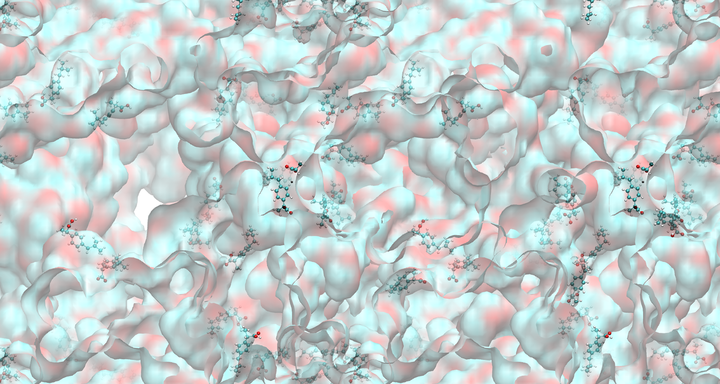
\includegraphics[width=0.47\linewidth]{img/ibu_s_100x_bp.png}}
	\hspace{0.2cm}
	\subfloat{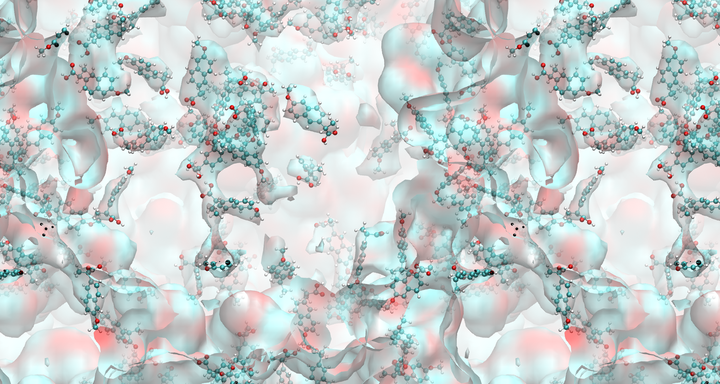
\includegraphics[width=0.47\linewidth]{img/nap_100x_bp.png}}\\
	\vspace{0.2cm}
	\subfloat{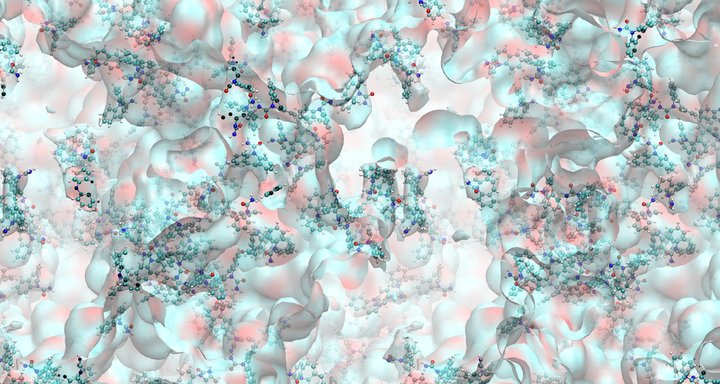
\includegraphics[width=0.47\linewidth]{img/cbz_100x_bp.png}}
	\hspace{0.2cm}
	\subfloat{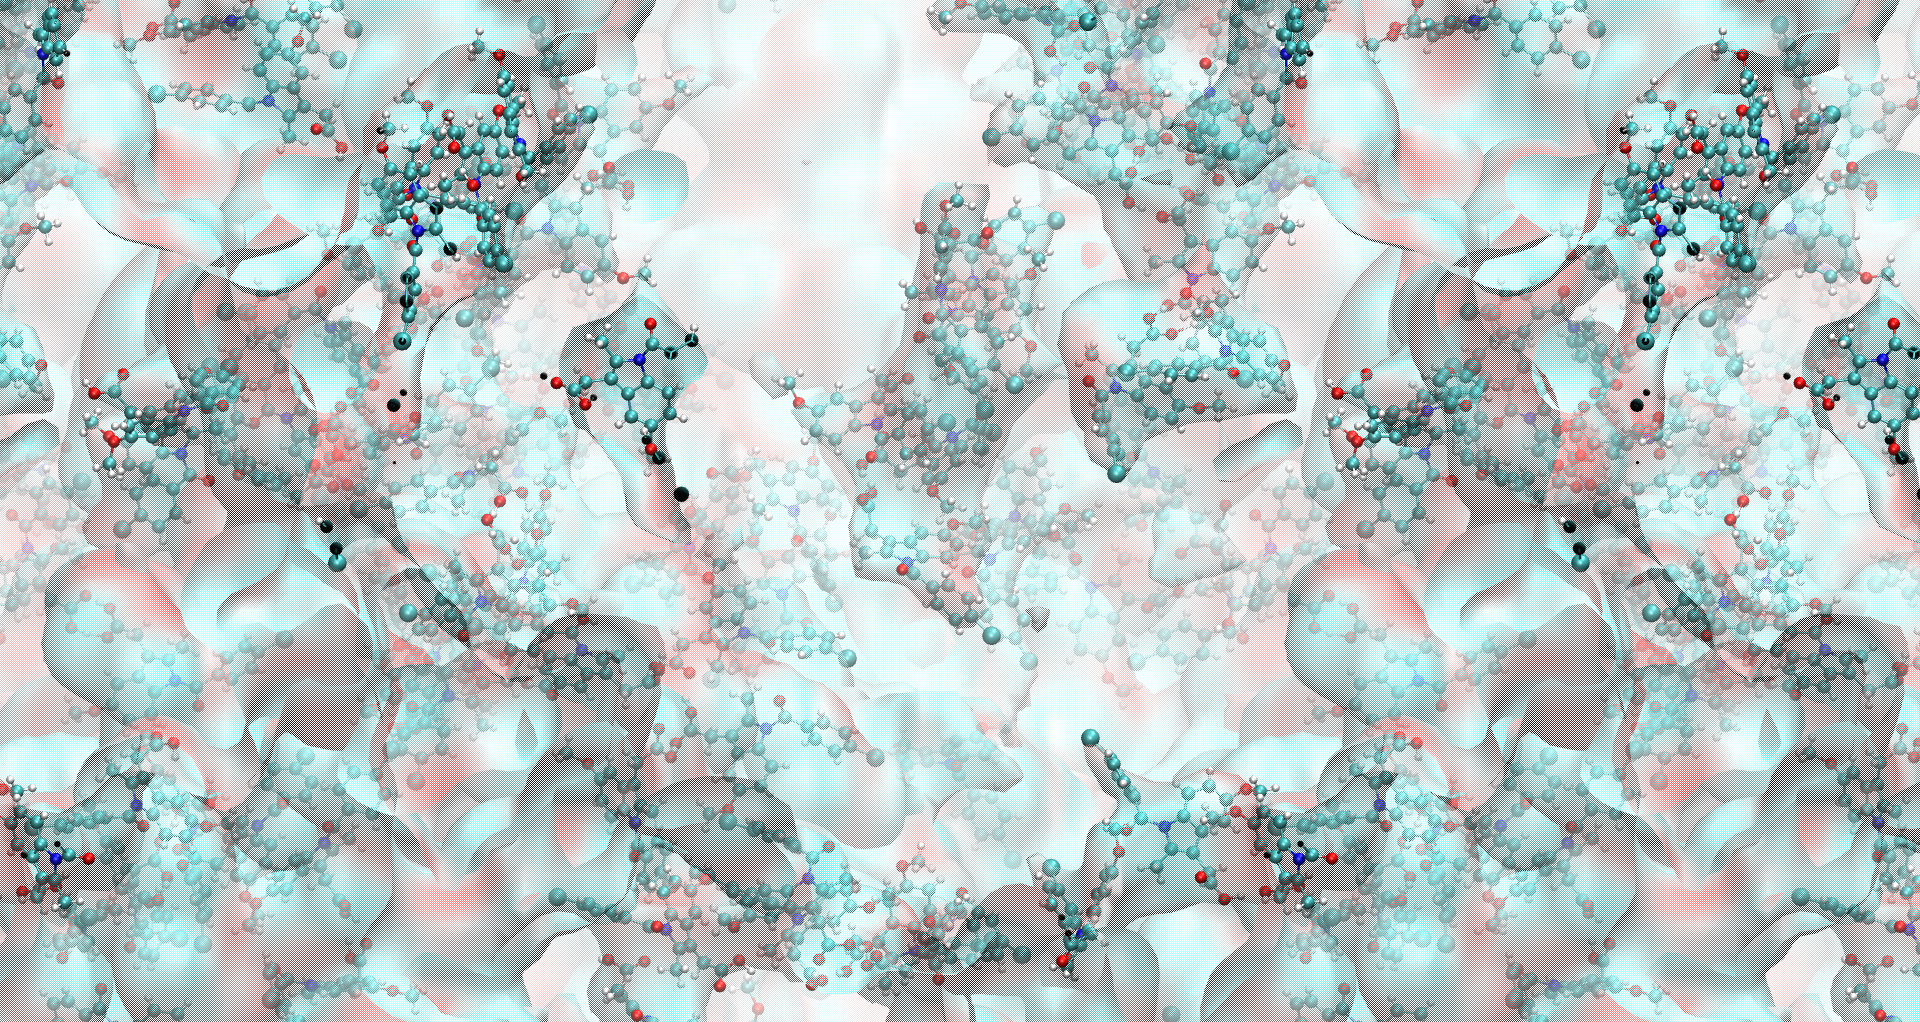
\includegraphics[width=0.47\linewidth]{img/indo_100x_bp.png}}
	\caption{Image of the simulation box for $x_{\text{API}}=0.85$ and $T=500~K$ for ibuprofen (\textbf{top left}), naproxen (\textbf{top right}), carbamazepine (\textbf{bottom left}) and indomethacin (\textbf{bottom right}).}
	\label{fig:mix_boxes}
\end{figure}

\newpage
\subsubsection{Excess properties}
Excess molar energy and excess molar volume are thermodynamic quantities that quantify deviations from ideal behavior in solutions. Ideal solutions exhibit no interactions between components, resulting in linear relationships between the properties of the mixture and its composition. However, real solutions often deviate from ideal behavior due to the interactions between molecules such as hydrogen bonding or their steric composition.

The excess molar energy represents the additional energy per mole of mixture compared to an ideal solution at the same temperature, pressure, and composition. It accounts for the energy associated with interactions between molecules in the mixture, including both attractive and repulsive forces. Positive excess molar energies indicate favorable interactions (hydrogen bonding), while negative values suggest repulsive interactions.

Similarly, the excess molar volume quantifies the deviation in volume per mole of mixture from that of an ideal solution. It reflects the changes in volume resulting from interactions between molecules, such as volume contraction due to strong molecular association or volume expansion due to repulsive interactions.

Excess molar volumes ($V^{E})$ of the mixtures were evaluated from the simulations for each concentration using the Equation \ref{eq:VM}. For this reason, the average molar volumes of the simulation boxes were evaluated from simulations of pure API ($V_{\text{m}}^{\text{API}} $) and pure polymer ($V_{\text{m}}^{\text{PLA}}$) and from a mixture ($V_{\text{m}}^{\text{MIX}}$) of API and PLA. To obtain the uncertainties block averaging scheme and error propagation law was used.  

\begin{equation}\label{eq:VM}
	V^{E} = V_{\text{m}}^{\text{MIX}} - x_{\text{API}} V_{\text{m}}^{\text{API}} - x_{\text{PLA}} V_{\text{m}}^{\text{PLA}}
\end{equation}

Excess molar energies of the mixtures were evaluated in a similar way. The following Equation \ref{eq:EM} was used

\begin{equation}\label{eq:EM}
	E^\text{E} = E_{\text{m}}^{\text{MIX}} - x_{\text{API}} E_{\text{m}}^{\text{API}} - x_{\text{PLA}} E_{\text{m}}^{\text{PLA}},
\end{equation}

where $E_{\text{m}}^{\text{MIX}}$ is the average molar energy of the simulation box of the mixture, $E_{\text{m}}^{\text{API}}$ is the average molar energy of pure API, and $E_{\text{m}}^{\text{PLA}}$ is the averaged molar energy of pure PLA obtained from simulation. Mixing energies and volumes were calculated for all systems and both temperatures (300, 500~K), and the comparison is shown in Table \ref{tab:vobjemy}.  

\begin{table}[htb]
	\caption{Calculated excess energies (kJ mol$^{-1}$) and volumes (in cm$^3$ mol$^{-1}$) for API mixtures of different concentrations from simulations under 300~K ($V_{300}^\text{E}$, $E_{300}^\text{E}$) and 500~K ($V_{500}^\text{E}$, $E_{500}^\text{E}$) with their standard uncertainties (k=1).}
	\centering
	\begin{tabular}{lSSSSSSSSS}
	\toprule
	\textbf{API} & \boldmath{$x_{\text{API}}$} & \boldmath{$V_{300}^\textbf{E}$} & \boldmath{$\sigma_{V^\textbf{E}}$} & \boldmath{$V_{500}^\textbf{E}$} & \boldmath{$\sigma_{V^\textbf{E}}$} & \boldmath{$E_{300}^\textbf{E}$} & \boldmath{$\sigma_{E^\textbf{E}}$} & \boldmath{$E_{500}^\textbf{E}$} & \boldmath{$\sigma_{E^\textbf{E}}$} \\
	\midrule
		cbz & 0.85 & 0 & 0 & 0.92 & 0.50 & 0 & 0 & 4.74 & 0.46 \\
		& 0.92 & 0 & 0 & 0.64 & 0.27 & 0 & 0 & 3.20 & 0.21 \\
		& 0.95 & 0 & 0 & 0.22 & 0.17 & 0 & 0 & 2.65 & 0.16 \\
		\midrule
		nap & 0.85 & 0 & 0 & 3.28 & 0.48 & 0 & 0 & 7.49 & 0.44 \\
		& 0.92 & 0 & 0 & 2.61 & 0.26 & 0 & 0 & 6.26 & 0.26 \\
		& 0.95 & 0 & 0 & 1.46 & 0.18 & 0 & 0 & 4.72 & 0.20 \\
		\midrule
		indo & 0.85 & 0 & 0 & -1.24 & 0.54 & 0 & 0 & 8.55 & 0.65 \\
		& 0.92 & 0 & 0 & -1.73 & 0.28 & 0 & 0 & 6.37 & 0.29 \\
		& 0.95 & 0 & 0 & -2.00 & 0.22 & 0 & 0 & 3.53 & 0.31 \\
		\midrule
		ibu & 0.85 & 0 & 0 & 0.25 & 0.49 & 0 & 0 & 3.28 & 0.42 \\
		& 0.92 & 0 & 0 & 0.11 & 0.29 & 0 & 0 & 2.63 & 0.24 \\
		& 0.95 & 0 & 0 & -0.14 & 0.17 & 0 & 0 & 2.12 & 0.15 \\
	\bottomrule
	\end{tabular}
	\label{tab:vobjemy} 
\end{table}

For higher temperature of 500~K all excess energies are positive, this indicate creating new intermolecular interactions between API and PLA in the mixtures. We can see, that for higher concentration of API in the mixture ($x_{\text{API}}$) the values of $E^\text{E}$ are decreasing also with their uncertainties. The reason could be that more interactions of API-API are still presented resulting in less populated API-PLA interactions that do not compensate the API-API cohesion. The analysis of radial distribution functions of the most favorable interactions between API-API and API-PLA was performed in order to see the which specific interactions are forming. Same trend was observed for the height of the first peak for different concentrations. Complete results are given in following section.

The excess volumes are also decreasing with higher concentration of API in the mixture. For carbamazepine and naproxen the $V^\text{E}$ values are positive, meaning less advantageous arrangement of molecules in space. For indomethacine all values are negative, more advantageous arrangement is observed. For ibuprofen the values are close to zero, for the highest API concentration the value is negative.

\subsubsection{Radial distribution functions}

Sampling the radial distribution function from the simulations was done to explore the interactions that are having the highest impact on material cohesion. The hydrogen bonds were mostly studied as the most important cohesive features. First the API-API contacts are discussed, then API-PLA interactions are studied.

The strongest API-API interaction was chosen and plotted to study the change between neat API and simulations of mixtures with different concentrations of PLA. For ibuprofen, naproxen and indomethacine the interaction between the oxygen and hydrogen atoms from carboxyl group was studied. However, carbamazepine does not contain complete carboxyl group, the hydrogen bonding was studied between the N$\text{H}_\text{2}$ and OC group. The selected atom types involved in interactions are visualised in the introduction section in Figure \ref{fig:APIs}. 

All RDFs of mixtures containing the API-API interaction were scaled onto the pure API RDF signal enabling us direct comparison of amplitudes of individual signals. The following Equation \ref{eq:RDF_formula} was used.

\begin{equation}\label{eq:RDF_formula}
	\text{RDF}_{\text{scaled}} = \text{RDF} \cdot \frac{V_{\text{API}}}{N_{\text{API}}} \frac{N_{\text{mix}}}{V_{\text{mix}}},
\end{equation}

where $V_{\text{API}}$ is the average volume of the pure API simulation box, $N_{\text{API}}$ is the number of molecules in the pure API simulation box and analogously for mixtures.

\newpage
\textbf{API-API interactions}

The RDF of the hydrogen bonding interaction in carboxyl group of indomethacin is shown in Figure \ref{fig:indo_RDF_}. The dimer of the carboxyl groups is the strongest in indomethacine in comparison to other studied APIs. The closest contact distance between O-H$\cdots$O is 1.5 \AA, with the first peak amplitude decreasing with less API in the mixture, for higher concentration of polymer in the mixture API-PLA interactions are more favorable. First coordination sphere contain one molecule, corresponding to the close dimer contact.

\begin{figure}[htb!]
	\centering
	\subfloat{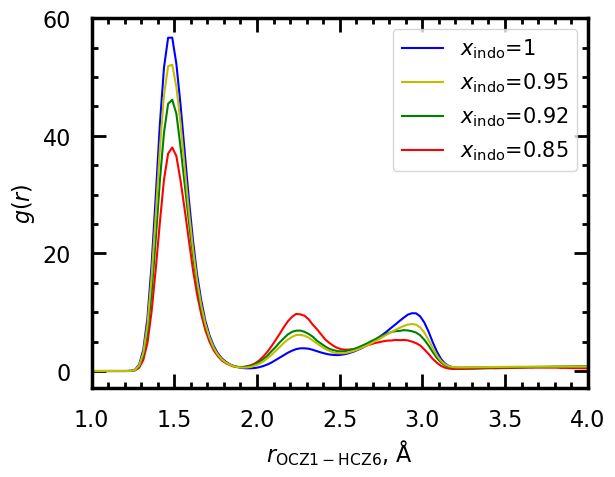
\includegraphics[width=0.4\linewidth]{img/rdf_indo_api_r1.png}}
	\subfloat{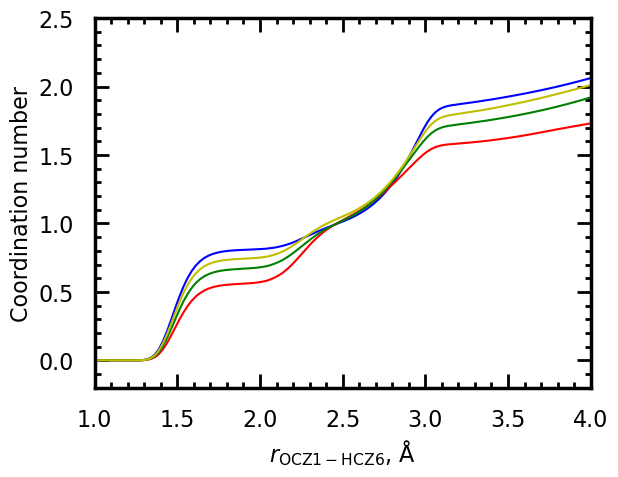
\includegraphics[width=0.4\linewidth]{img/coord_indo_api_r1.png}}\\
	\subfloat{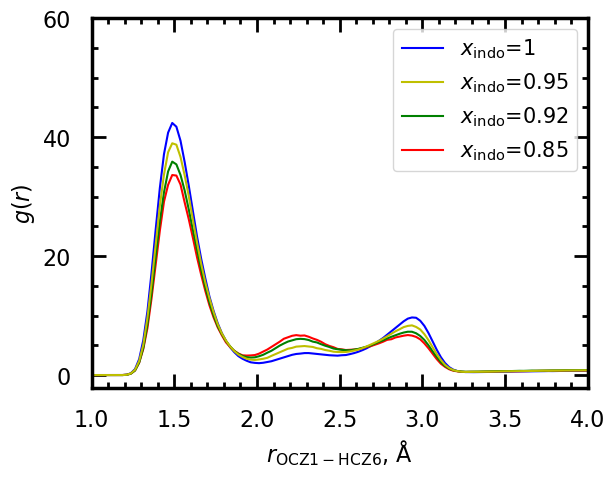
\includegraphics[width=0.4\linewidth]{img/rdf_indo_api_r2.png}}
	\subfloat{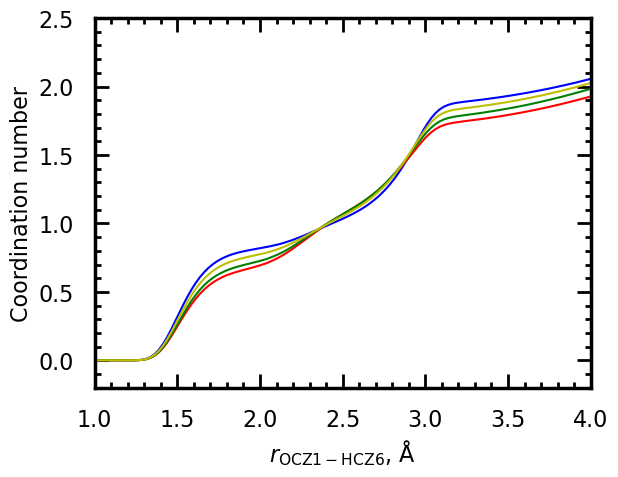
\includegraphics[width=0.4\linewidth]{img/coord_indo_api_r2.png}}
	\vspace{-0.3cm}
	\caption{RDF of the API-API interaction between HCZ6 hydrogen atom and OCZ1 oxygen atom from COOH group in a mixture of indo and PLA for different concentration normalized on values for pure indo, temperature of 300~K in the left upper corner and 500~K bottom left, coordination numbers on the right.}
	\label{fig:indo_RDF_}
\end{figure}


The RDFs of the interaction in carboxyl groups of naproxen and ibuprofen are shown in Figure \ref{fig:nap_RDF_} and \ref{fig:ibu_s_RDF_}. The contact distance of O-H$\cdots$O is 1.75 \AA~in both cases. We can observe interesting trend for both API. In pure API, the dimer is linked by two hydrogen bonds, corresponding to two massive peaks of the function. With the higher concentration of PLA in the mixture, the shape of the RDF is changing. This change resulted in higher probability of the contact at longer distances, meaning that APIs prefer looser contact of their COOH dimers. The reason for that could be that first sphere is taken by interaction of hydrogen from API with oxygens from PLA which happen on distances 2 and 4 \AA. This contact is described further in the next paragraphs. 


\newpage
\begin{figure}[H]
	\centering
	\subfloat{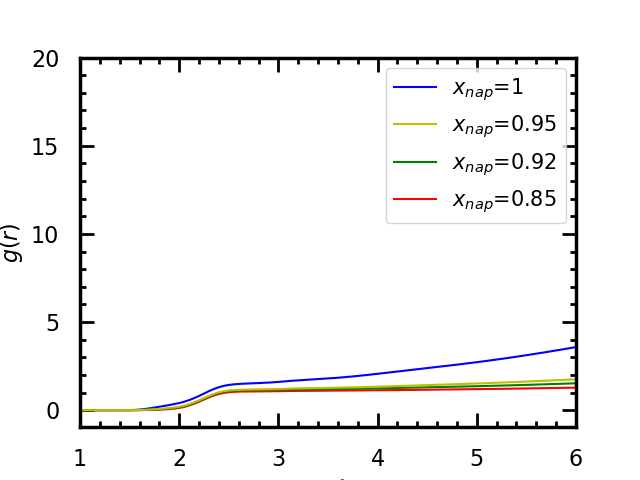
\includegraphics[width=0.4\linewidth]{img/rdf_nap_api_r1.png}}
	\subfloat{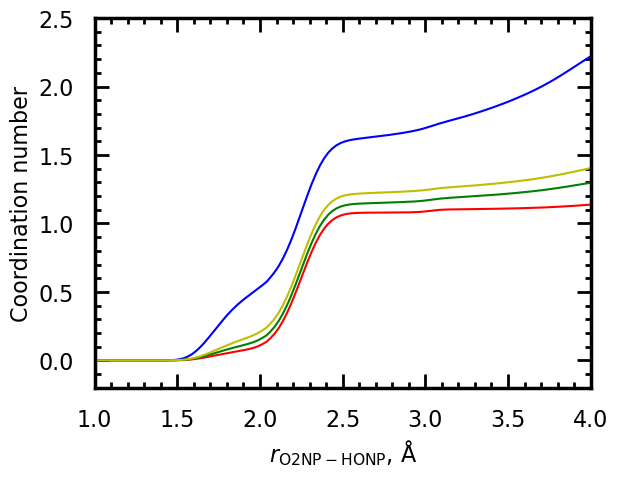
\includegraphics[width=0.4\linewidth]{img/coord_nap_api_r1.png}}\\
	\subfloat{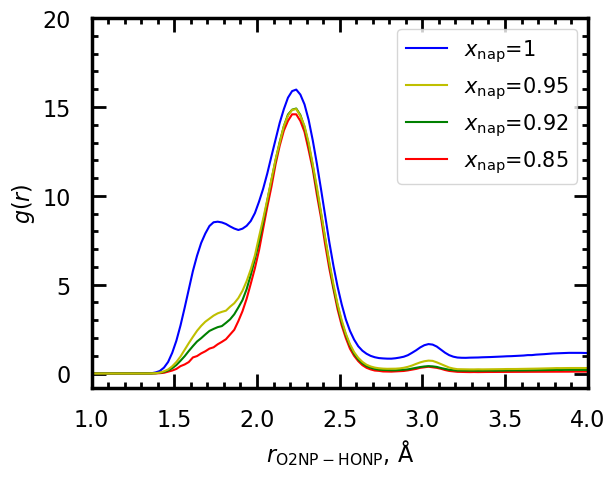
\includegraphics[width=0.4\linewidth]{img/rdf_nap_api_r2.png}}
	\subfloat{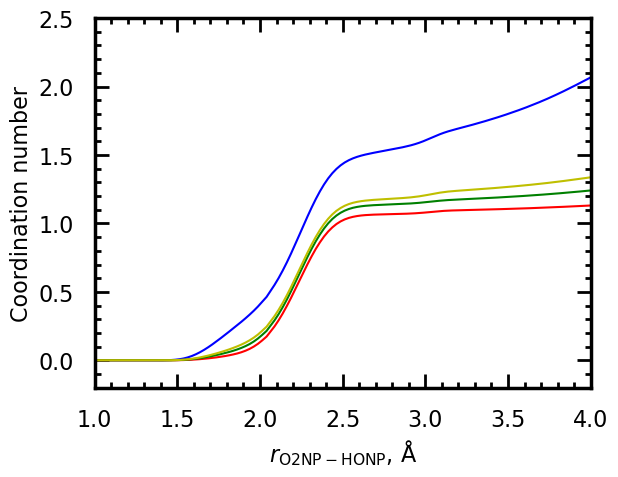
\includegraphics[width=0.4\linewidth]{img/coord_nap_api_r2.png}}
	\vspace{-0.3cm}
	\caption{RDF of the API-API interaction between HONP hydrogen atom and O2NP oxygen atom from COOH group in a mixture of nap and PLA for different concentration normalized on values for pure nap, temperature of 300~K in the left upper corner and 500~K bottom left, coordination numbers on the right.}
	\label{fig:nap_RDF_}
\end{figure}

\begin{figure}[H]
	\centering
	\subfloat{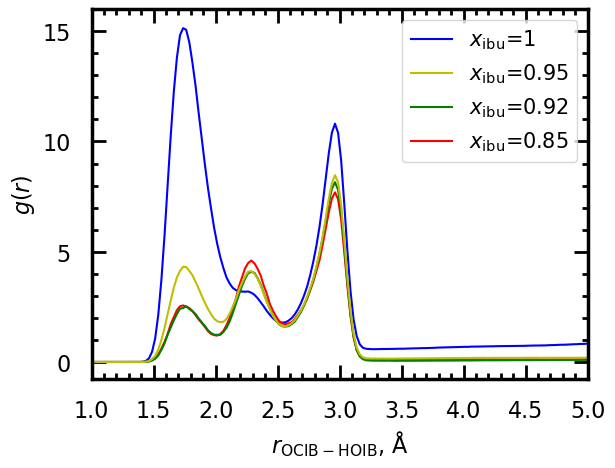
\includegraphics[width=0.4\linewidth]{img/rdf_ibu_s_api_r1.png}}
	\subfloat{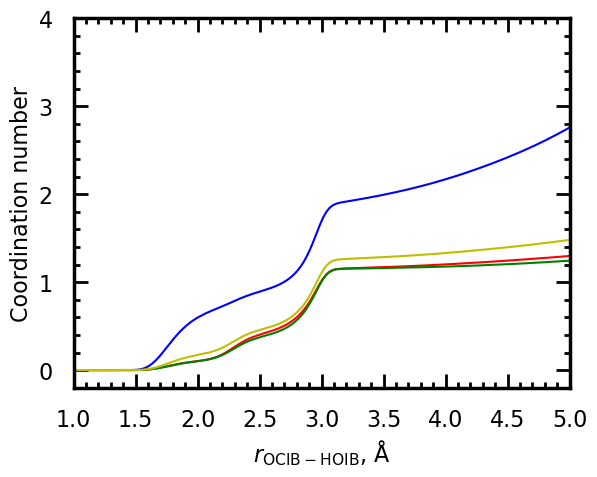
\includegraphics[width=0.39\linewidth]{img/coord_ibu_s_api_r1.png}} \\
	\subfloat{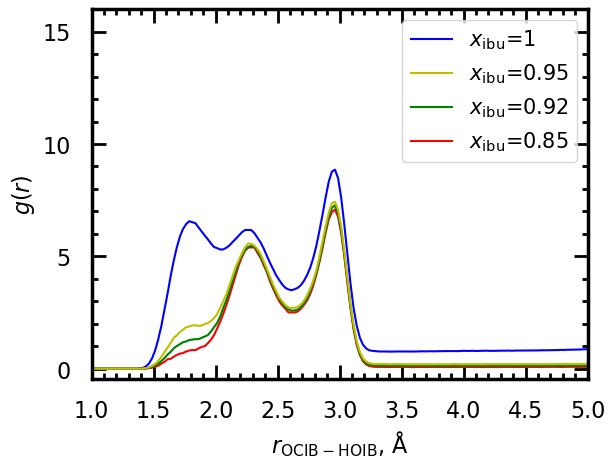
\includegraphics[width=0.4\linewidth]{img/rdf_ibu_s_api_r2_15.png}}
	\subfloat{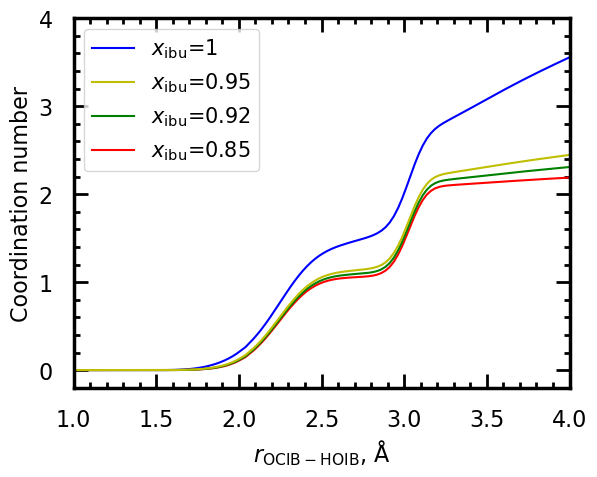
\includegraphics[width=0.39\linewidth]{img/coord_ibu_s_api_r2.png}}
	\vspace{-0.3cm}
	\caption{RDF of the API-API interaction between carboxyl HOIB hydrogen atom and OCIB oxygen atom in a mixture of ibu and PLA for different concentration normalized on values for pure ibu, temperature of 300~K in the left upper corner and 500~K bottom left, coordination numbers on the right.}
	\label{fig:ibu_s_RDF_}
\end{figure}

\newpage
The RDF of the hydrogen bonding interaction of carbamazepine is shown in Figure \ref{fig:cbz_RDF_}. There are two peaks presented, that correspond to interactions of 2 equivalent hydrogen atoms bonded on nitrogen, each participating the same linking the dimer with 2 hydrogen bonds. The contact distance O-H$\cdots$O is 2.25 \AA. The shape and signal response of the peaks is similar for neat API and  mixtures for both temperatures. There is almost no change between different concentration of API, meaning that the impact of PLA on the cohesion of carbamazepine in the mixture is very low.


\begin{figure}[htb]
	\centering
	\subfloat{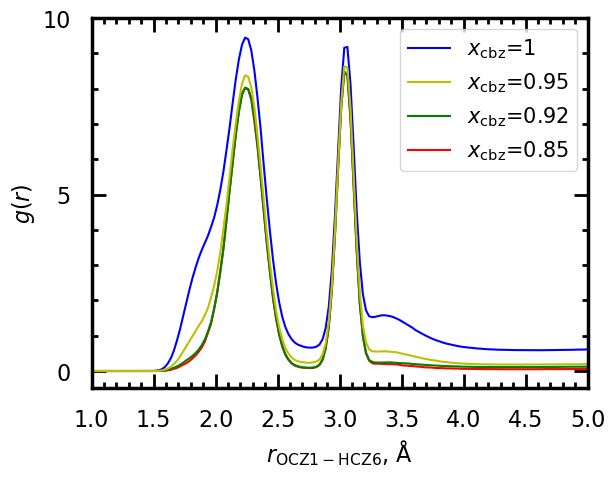
\includegraphics[width=0.4\linewidth]{img/rdf_cbz_api_r1.png}}
	\subfloat{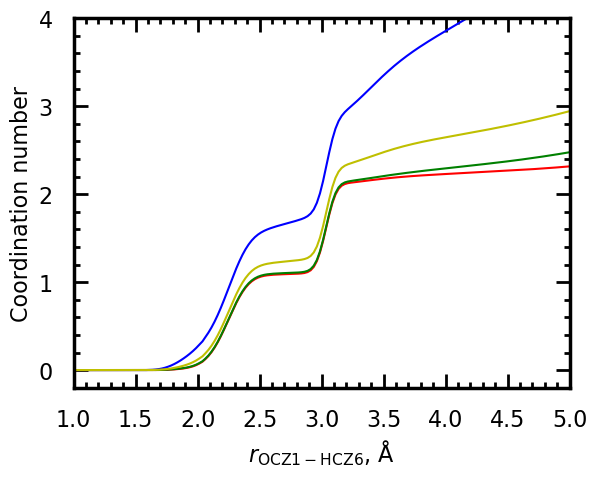
\includegraphics[width=0.39\linewidth]{img/coord_cbz_api_r1.png}}\\
	\subfloat{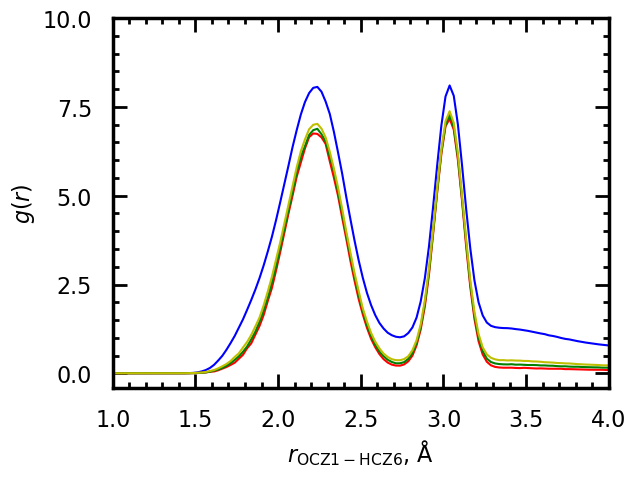
\includegraphics[width=0.4\linewidth]{img/rdf_cbz_api_r2.png}}
	\subfloat{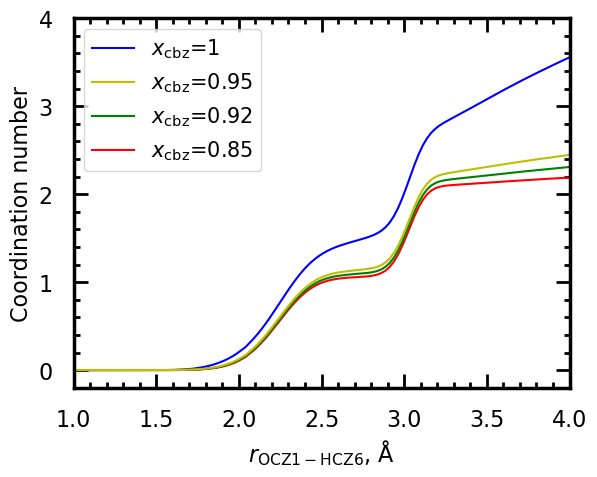
\includegraphics[width=0.39\linewidth]{img/coord_cbz_api_r2.png}}
	\vspace{-0.3cm}
	\caption{RDF of the API-API interaction between HCZ6 hydrogen atom bonded on nitrogen and OCZ1 oxygen atom in a mixture of cbz and PLA for different concentration normalized on values for pure cbz, temperature of 300~K in the left upper corner and 500~K bottom left, coordination numbers on the right.}
	\label{fig:cbz_RDF_}
\end{figure}


\newpage
\textbf{API-PLA interactions}

In this part we are focusing on the hydrogen bonding between API and PLA, where API acts as a donor of hydrogen and PLA as its acceptor. Optimization of the conformation was performed for each dimer composed of two units long PLA chain and one API molecule using quantum methods in Gaussian\cite{frisch_gaussian16_2016} software by B3LYP functional with the 6-31+g(d,p) basis set with the dispersion correction GD3BJ \cite{smith_revised_2016}. The optimized configuration with studied atom types marked is available in Figure~\ref{fig:contact}.
\vspace{-0.3cm}
\begin{figure}[htb!]
	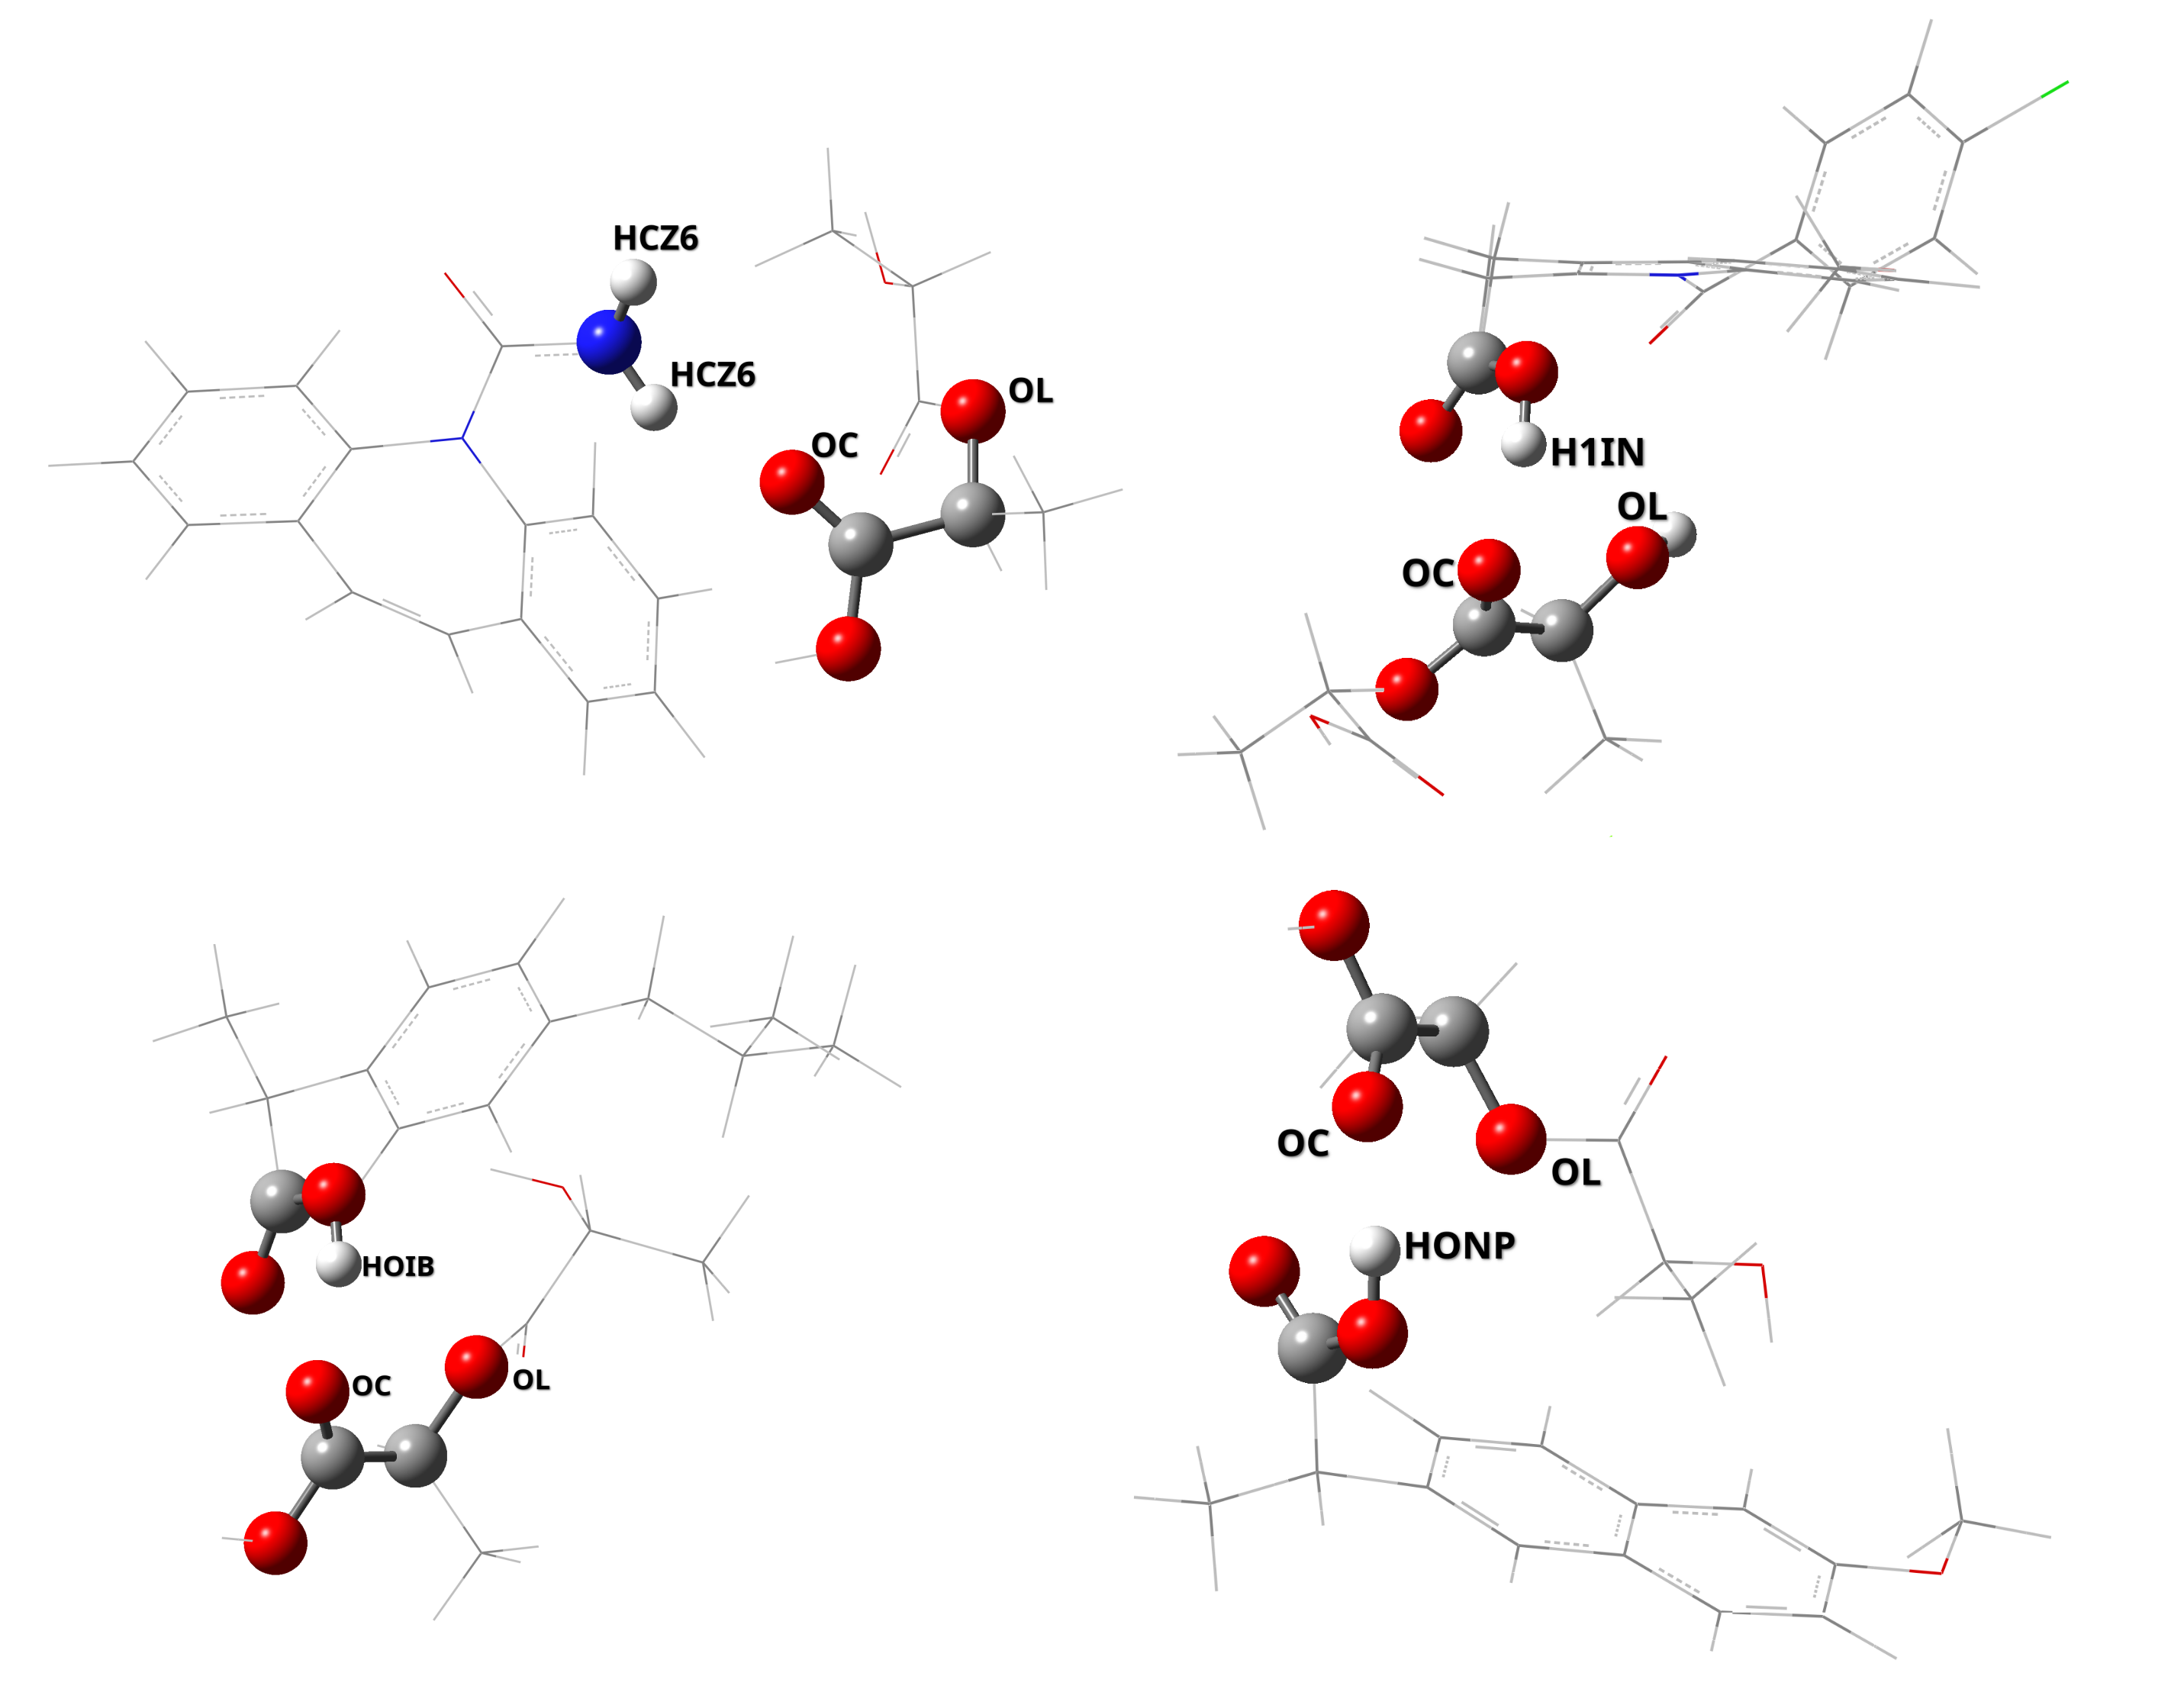
\includegraphics[width=\linewidth]{img/all_pla_api_bp.png} 
	\vspace{-1cm}
	\caption{Visualization of the interaction between hydrogen atom from API and oxygen atom from PLA with marked atom types involved. Carbamazepine (\textbf{top left}), indomethacin (\textbf{top right}), ibuprofen (\textbf{bottom left}) and naproxen (\textbf{bottom right}).}
	\vspace{-0.3cm}
	\label{fig:contact}    
\end{figure}


The RDF of hydrogen bonding with the carbonyl group in PLA (OC) is shown in Figure \ref{fig:carbonyl}. The RDF value converges to one in a long distance for all API-PLA interactions, which is in good agreement with theory. For indomethacine, the amplitude of the peak decrease with lower PLA molecules presented in the mixture. This correspond with the observation for trends in INDO-INDO interactions. The contact distance in dimer obtained from quantum optimization is 1.76 \AA, from MD simulation we obtained the value of \AA.


For carbamazepine, there are two peaks in the RDF function. The peaks corresponding to those interactions are weak, we can see that the intensity of the peaks is really low. Under temperature 300 K the intensity of the first peak is slightly above one, but for 500 K the first peak is below one, meaning that this interaction occurs less at a small distance than in the rest of the system. The impact of the PLA concentration change is not that visible, especially for higher temperature of 500~K. This also correspond to we saw in the CBZ-CBZ interactions. The contact distance value from quantum calculations is 2.01 \AA, which is the same as the distance of first RDF obtained by MD.


The hydrogen bonds with the oxygen bonded by ether bond in PLA structure are shown in Figure \ref{fig:ether}. All values also converge to 1 in a long distance for all APIs. Generally, those interactions are much weaker than those with oxygen from carbonyl group. 

\newpage
\begin{figure}[H]
	\centering
	\subfloat{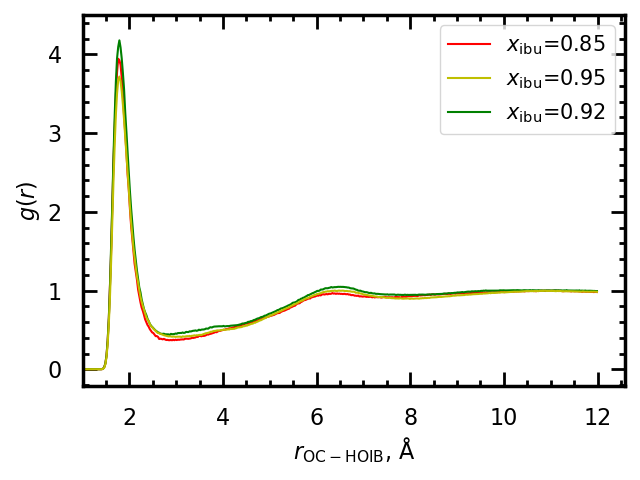
\includegraphics[width=0.5\linewidth]{img/RDF_ibu_s_20_2.png}}
	\subfloat{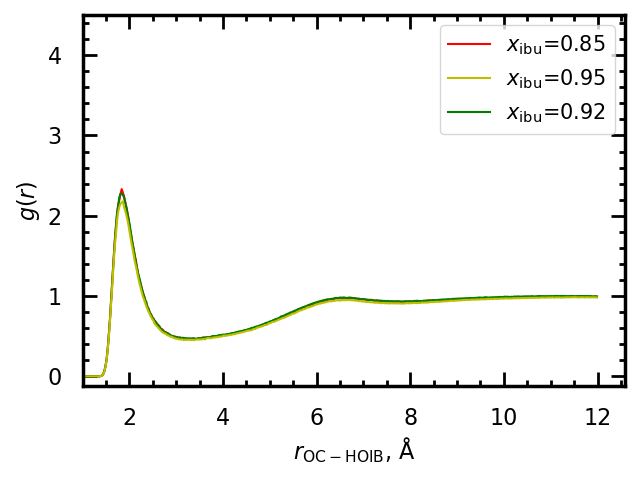
\includegraphics[width=0.5\linewidth]{img/RDF_ibu_s_20_2_r2.png}}\\
	\vspace{-0.2cm}
	\subfloat{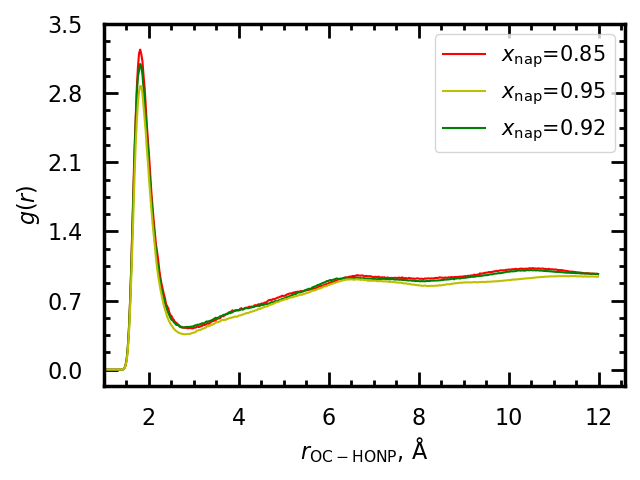
\includegraphics[width=0.5\linewidth]{img/RDF_nap_2_31.png}}
	\subfloat{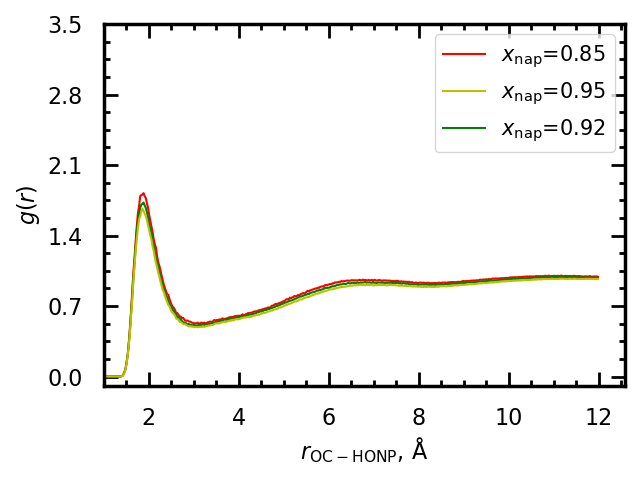
\includegraphics[width=0.5\linewidth]{img/RDF_nap_2_31_r2.png}}\\
	\vspace{-0.2cm}
	\subfloat{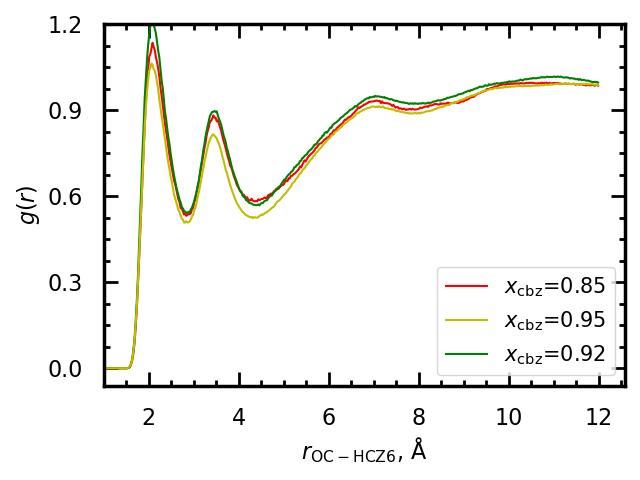
\includegraphics[width=0.5\linewidth]{img/RDF_cbz_2_27.png}}
	\subfloat{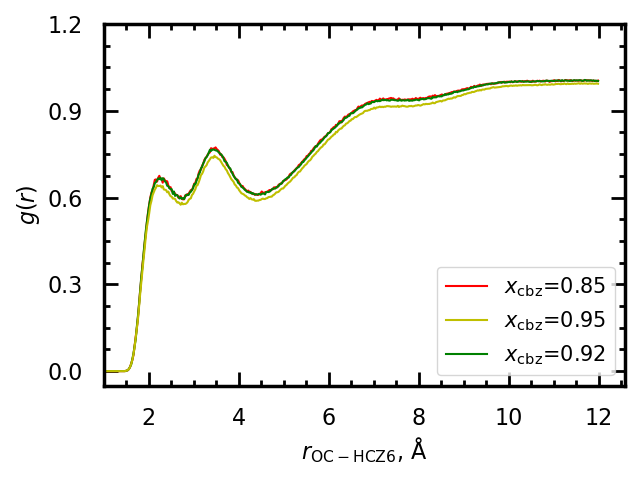
\includegraphics[width=0.5\linewidth]{img/RDF_cbz_2_27_r2.png}}\\
	\vspace{-0.2cm}
	\subfloat{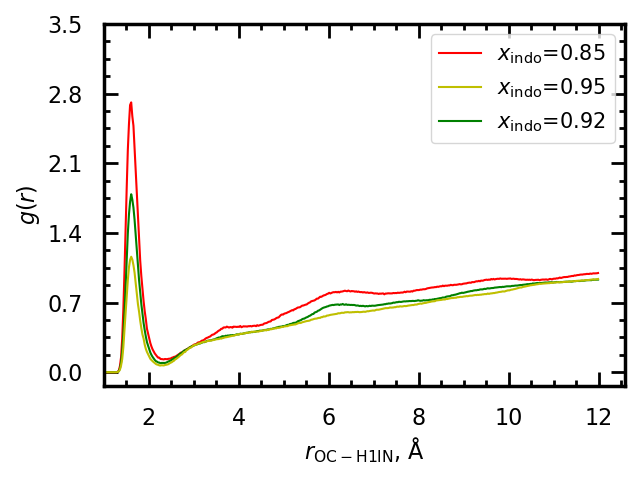
\includegraphics[width=0.5\linewidth]{img/RDF_indo_2_36.png}}
	\subfloat{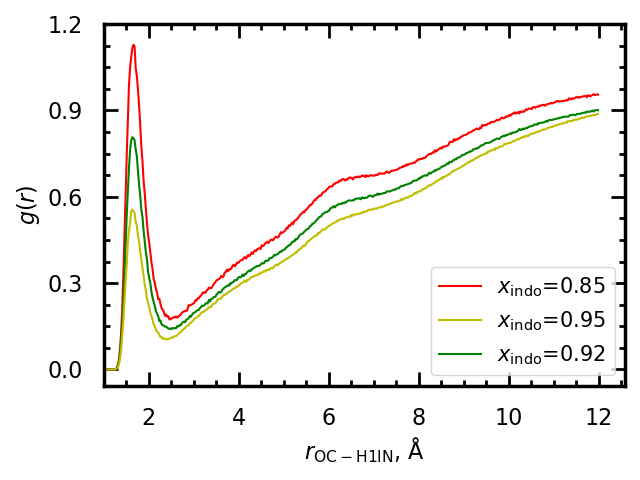
\includegraphics[width=0.5\linewidth]{img/RDF_indo_2_36_r2.png}}
		\vspace{-0.2cm}
	\caption{Radial distribution function of the interaction between hydrogen atoms and oxygen atom from carbonyl group in PLA, first ibuprofen on top, second naproxen, third carbamazepine and indomethacine in the bottom, temperature 300~K on the left and 500~K on the right.}
	\label{fig:carbonyl}
\end{figure}

\newpage
\begin{figure}[H]
	\centering
	\subfloat{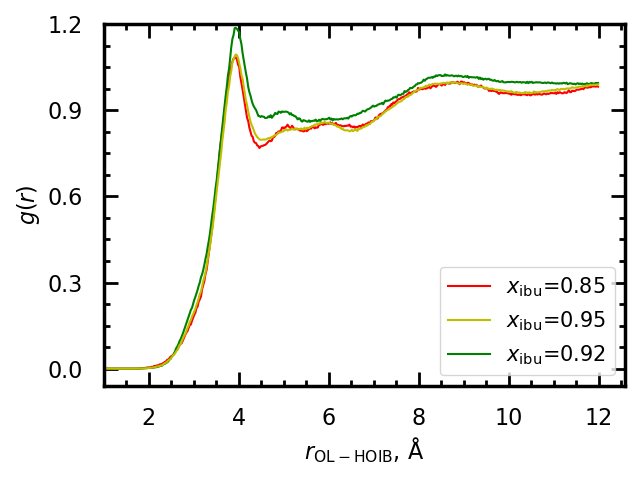
\includegraphics[width=0.5\linewidth]{img/RDF_ibu_s_20_6.png}}
	\subfloat{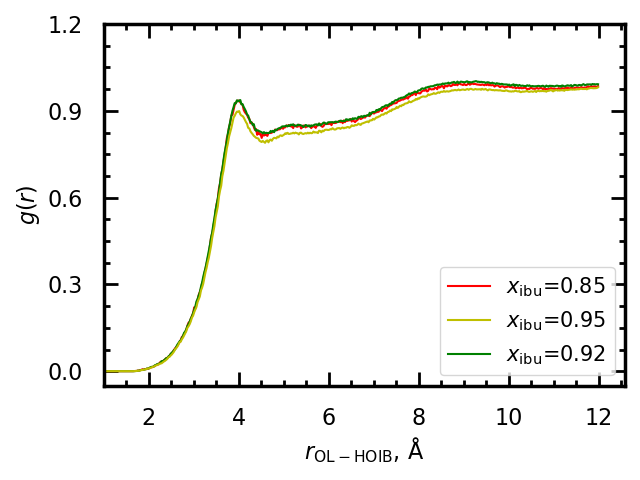
\includegraphics[width=0.5\linewidth]{img/RDF_ibu_s_20_6_r2.png}}\\
	\vspace{-0.2cm}
	\subfloat{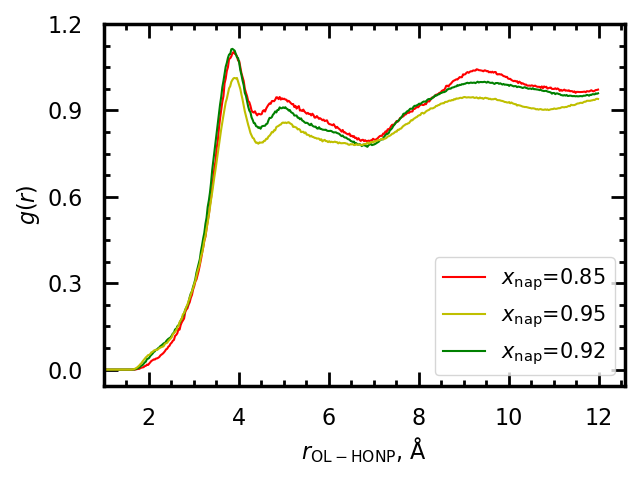
\includegraphics[width=0.5\linewidth]{img/RDF_nap_6_31.png}}
	\subfloat{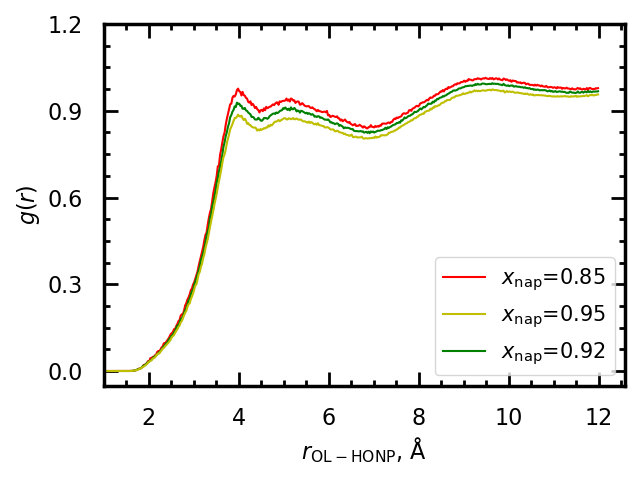
\includegraphics[width=0.5\linewidth]{img/RDF_nap_6_31_r2.png}}\\
	\vspace{-0.2cm}
	\subfloat{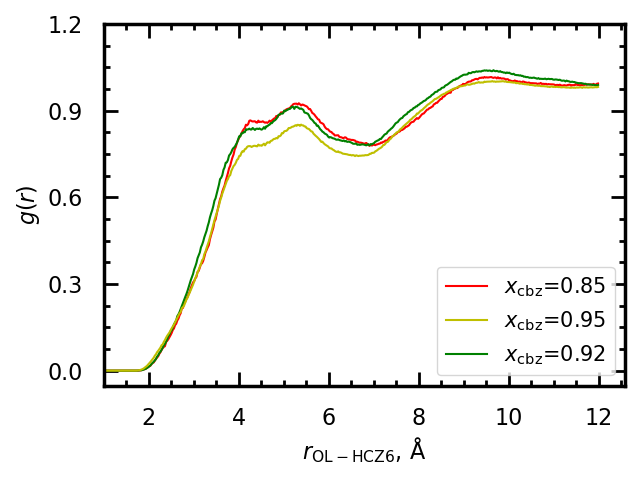
\includegraphics[width=0.5\linewidth]{img/RDF_cbz_6_27.png}}
	\subfloat{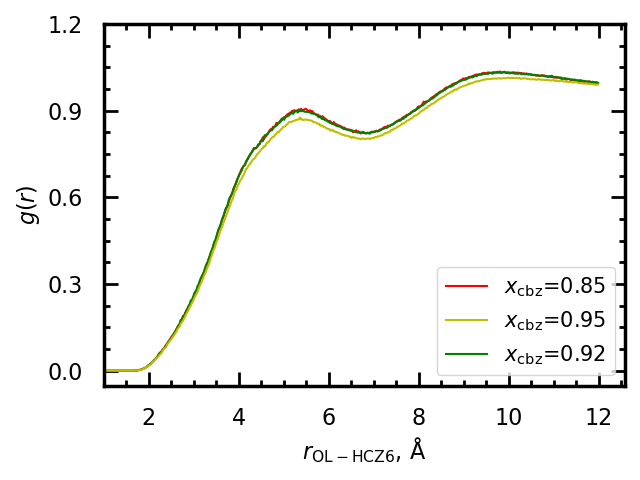
\includegraphics[width=0.5\linewidth]{img/RDF_cbz_6_27_r2.png}}\\
	\vspace{-0.2cm}
	\subfloat{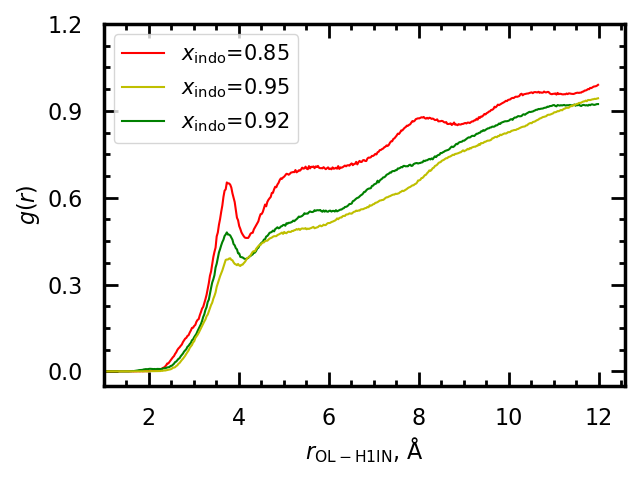
\includegraphics[width=0.5\linewidth]{img/RDF_indo_36_6.png}}
	\subfloat{\includegraphics[width=0.5\linewidth]{img/RDF_indo_36_6_r2.png}}
	\vspace{-0.2cm}
	\caption{Radial distribution function of the interaction between hydrogen atoms and oxygen atom bonded by ether bond in PLA, first ibuprofen on top, second naproxen, third carbamazepine and indomethacine in the bottom, temperature 300~K on the left and 500~K on the right.}
	\label{fig:ether}
\end{figure}

\newpage
\subsubsection{Diffusion coefficients}
The MSDs were sampled from the 10~ns long run simulations every 1000 fs (integration step 1 fs). At each sampled time step, obtained MSD data were averaged over all API molecules and then plotted as a function of the simulation time. The MSD dependencies were then interpolated by linear functions and related self-diffusivities of the API in the mixtures were evaluated from the slope of the line using the following Equation \ref{eq:D} obtained by modifying the Einstain equation from the theoretical part.

\begin{equation}\label{eq:D}
	D_{\text{API}} = \frac{a}{6}, 
\end{equation}
where $D$ is the diffusion coefficient, $a$ is the slope of the line.

The MSD data for APIs in mixtures with PLA for $T$=500~K are plotted in Figure \ref{fig:msd_r2}. For ibuprofen, there is a significant difference between mobility of neat API and API mixed within the polymer. This could be result of very strong API-PLA interaction forming in the mixture. The data of carbamazepine shows that with increasing API concentration, mobility also increases. There is also not that enormous difference between neat API. For naproxen, it seems that there is no change for different concentrations of mixtures, also in neat API the mobility is higher. The situation for indometacine is completely different. For neat API the mobility is really low compared to mixtures with PLA. This behaviour seems strange, the reason could be, that in pure API, there are really strong API-API interactions that decrease the mobility. Also the MSD values are much lower.

\begin{figure}[]
	\centering
	\subfloat{\includegraphics[width=0.4\linewidth]{img/msd_cbz_api_r2.png}}
	\subfloat{\includegraphics[width=0.4\linewidth]{img/msd_nap_api_r2.png}}\\
	\subfloat{\includegraphics[width=0.4\linewidth]{img/msd_ibu_s_api_r2.png}}
	\subfloat{\includegraphics[width=0.4\linewidth]{img/msd_indo_api_r2.png}} 
	\caption{MSD from simulations under 500 K, ibuprofen (\textbf{top left}), naproxen (\textbf{top right}), carbamazepine (\textbf{bottom left}) and indomethacin (\textbf{bottom right}).}
	\label{fig:msd_r2}    
\end{figure}

\newpage
Self-diffusivities were evaluated from the above data and plotted in Figure \ref{fig:d}. The data reveal that in pure liquid carbamazepine the diffusion is faster than in naproxen. For higher temperatures, the main factor affecting diffusion is the shape of the molecules, not the strength of the intermolecular interactions. This is caused because the kinetic energy is higher than the potential for higher temperatures.
\begin{figure}[htb!]
	\centering
	\includegraphics[width=0.4\linewidth]{img/d_coeficienty.png} 
	\caption{Self-diffusivities for carbamazepine and naproxen as a function of their concentration in the mixtures, temperature 500 K.}
	\label{fig:d}    
\end{figure}  

MSD was also evaluated at a lower temperature of 300 K, Figure \ref{fig:msd_r1}. There is the opposite trend. From these data sets, we can assume that carbamazepine has lower interactions with polymer because the mobility in the mixtures is higher than that in the pure state. The mobility of naproxen is always lower in mixtures, which is related to its stronger interactions with the polymer. The strength of the intermolecular interactions has a greater impact, meaning that paired molecules NAP-API slow the diffusion of other particles.

\begin{figure}[]
	\centering
	\subfloat{\includegraphics[width=0.4\linewidth]{img/msd_cbz_api_r1.png}}
	\subfloat{\includegraphics[width=0.4\linewidth]{img/msd_nap_api_r1.png}}\\
	\subfloat{\includegraphics[width=0.4\linewidth]{img/msd_ibu_s_api_r1.png}}
	\subfloat{\includegraphics[width=0.4\linewidth]{img/msd_indo_api_r1.png}} 
	\caption{MSD from simulations under 300 K, ibuprofen (\textbf{top left}), naproxen (\textbf{top right}), carbamazepine (\textbf{bottom left}) and indomethacin (\textbf{bottom right}).}
	\label{fig:msd_r1}    
\end{figure}

\subsubsection{Glass transition temperature}
The glass transition temperatures of the mixtures were evaluated from the simulated annealing runs by fitting a hyperbola to the temperature-density data. The whole methodology is described in the paper written by Alzate-Vargas et al.\cite{alzate-vargas_uncertainties_2018}, the main equation of the fit is Equation \ref{eq:fit}

\begin{equation}\label{eq:fit}
	\rho(T)=\rho_0-a\left(T-T_0\right)-b\left[\frac{1}{2}\left(T-T_0\right)+\sqrt{\frac{\left(T-T_0\right)^2}{4}+e^c}\right].
\end{equation}

Since this method is sensitive to the initial state of the simulated box, more simulated data starting from different conformations must be provided to evaluate $T_\text{g}$ with the information about its uncertainty. In this work we used 5 simulations from different initial states obtained from 5~ns long run sampled each nanosecond.

TO DO: DOPOČÍTAT PRO NOVÉ SIMULACE
\begin{table}[htb!]
	\caption{Calculated glass transition temperatures $T_\text{g}$ of mixtures composed from API and PLA with concentration of $x$=0.85 and their standard uncertainties.}
	\centering
	\begin{tabular}{lcc} \toprule
		{\textbf{API}} & {\textbf{\boldmath{$T_{\text{g}}$}}} & \textbf{{\boldmath{$\sigma_{T_\text{g}}$}}} \\
		\midrule
		carbamazepine  & 0 & 0 \\		
		naproxen   & 0 & 0 \\
		ibuprofen  & 0 & 0 \\
		indometacine  & 0 & 0 \\
		\bottomrule
	\end{tabular}
	\label{tab:Tg_mix} 
\end{table} 

